
%---------------------Slide 3--------------------------
%\begin{section}{Introducci\'on}
%	\begin{frame}
%		\frametitle{Vector Autoregressive Models}
\section{Vector Autoregressive Models}
\subsection{Introducci\'on}
		Desde la cr\'{\i}tica de Sims \cite{sims1980macroeconomics} a principios de los años ochenta del siglo pasado, el an\'alisis multivariado de datos, en el contexto de los modelos autorregresivos vectoriales (en adelante, VAR por su sigla en ingl\'es  \textbf{Vector Autoregressive Models}) se ha transformado en un instrumento est\'andar en econometr\'{\i}a. \\
		Debido a que las pruebas estad\'{\i}sticas se utilizan con frecuencia para determinar interdependencias y relaciones din\'amicas entre variables, esta metodolog\'{\i}a pronto se enriqueci\'o al incorporar información antes no considerada.\\	
%	\end{frame}
	%---------------------------------------------------------
	%---------------------Slide 4--------------------------
%	\begin{frame}
%		\frametitle{Vector Autoregressive Models}	
		Los modelos VAR explican las variables end\'ogenas \'unicamente por su propia historia, adem\'as de los regresores determin\'{\i}sticos. En contraste, los modelos VAR estructurales (en adelante, SVAR, por Structural VAR) permiten el modelado expl\'{\i}cito de la interdependencia contempor\'anea entre las variables del lado izquierdo. Por lo tanto, este tipo de modelos intenta eludir las deficiencias de los modelos VAR.\\
%	\end{frame}
	%---------------------------------------------------------
	%---------------------Slide 5--------------------------
%	\begin{frame}
%		\frametitle{Vector Autoregressive Models}
		Un VAR es un sistema de dos o m\'as series de tiempo que se modela considerando rezagos de las variables y la interacción din\'amica que pudiera existir entre ellas. Consiste fundamentalmente de dos dimensiones, el n\'umero de variables (g) y el n\'umero de rezagos (k). El caso más simple es un VAR bivariado:
		
		\begin{equation*}
		y_{1t} = \beta_{10} + \beta_{11} y_{1t-1} + \dots{} +  \beta_{1k} y_{1t-k} + \alpha_{11} y_{2t-1} + \dots{} +  \alpha_{1k} y_{2t-k} + \mu_1t
		\end{equation*}
		\begin{equation*}
		y_{2t} = \beta_{20} + \beta_{21} y_{2t-1} + \dots{} +  \beta_{2k} y_{2t-k} + \alpha_{21} y_{1t-1} + \dots{} +  \alpha_{2k} y_{1t-k} + \mu_2t
		\end{equation*}
		
		donde $u_{it}$ es un t\'ermino de error con $E(u_{it})=0$, $i =1,2$; $E(u_{1t} u_{2t})=0$. El supuesto de independencia de los errores puede relajarse como veremos m\'as adelante.
		
		El an\'alisis podr\'{\i}a extenderse por ejemplo a un modelo VAR (g), donde tenemos g variables y g ecuaciones.
		
%	\end{frame}
%\end{section}
%---------------------------------------------------------
%---------------------Slide 6--------------------------
%\begin{section}{Notaci\'on y Conceptos}
%	\begin{frame}
%		\frametitle{Vector Autoregressive Models}
\pagebreak\subsection{Notaci\'on y Conceptos}
		Una caracter\'{\i}stica importante de los modelos VAR es la sencillez de su notaci\'on. Por ejemplo, considere el caso de arriba, donde k = 1. Podemos escribir este modelo como:
		\begin{equation*}
		y_{1t} = \beta_{10} + \beta_{11} y_{1t-1} + \alpha_{11} y_{2t-1} + \mu_1t
		\end{equation*}
		\begin{equation*}
		y_{2t} = \beta_{20} + \beta_{21} y_{2t-1} + \alpha_{21} y_{1t-1} + \mu_2t
		\end{equation*}
		
		\'o
		
		\begin{gather}
		\begin{pmatrix} y_{1t} \\ y_{2t} \end{pmatrix}
		=
		\begin{pmatrix} \beta_{10} \\ \beta_{20} \end{pmatrix}
		+
		\begin{pmatrix} \beta_{11} & \alpha_{11} \\ \alpha_{21} & \beta{21} \end{pmatrix}
		\begin{pmatrix} y_{1t-1} \\ y_{2t-1} \end{pmatrix}
		+
		\begin{pmatrix} \mu_{1t} \\ \mu_{2t} \end{pmatrix}
		\end{gather}
		
		o incluso de forma m\'as compacta como
		
		\begin{gather}
		\begin{matrix} y_{t} =       \\ g x 1 \end{matrix}
		\begin{matrix} \beta_{0} +\\ g x 1 \end{matrix}
		\begin{matrix} \beta_{1}   \\ g x g \end{matrix}
		\begin{matrix} y_{t-1} +    \\ g x 1 \end{matrix}
		\begin{matrix} \mu_{1t}    \\ g x 1 \end{matrix}
		\end{gather}
		
%	\end{frame}
	%---------------------------------------------------------
	%---------------------Slide 7--------------------------
%	\begin{frame}
%		\frametitle{Vector Autoregressive Models}
		Este modelo se puede extender al caso en que hay $k$ retardos de cada variable en cada ecuaci\'on:
		
		\begin{gather}
		\begin{matrix} y_{t} =       \\ g x 1 \end{matrix}
		\begin{matrix} \beta_{0} +\\ g x 1 \end{matrix}
		\begin{matrix} \beta_{1}   \\ g x g \end{matrix}
		\begin{matrix} y_{t-1} +    \\ g x 1 \end{matrix}
		\begin{matrix} \beta_{2}   \\ g x g \end{matrix}
		\begin{matrix} y_{t-2} +    \\ g x 1 \end{matrix}
		\begin{matrix} \dots{}    \\  \end{matrix}
		\begin{matrix} \beta_{k}   \\ g x g \end{matrix}
		\begin{matrix} y_{t-k} +    \\ g x 1 \end{matrix}
		\begin{matrix} \mu_{1t}    \\ g x 1 \end{matrix}
		\end{gather}
		
		Tambi\'en podemos extender este al caso en que el modelo incluye t\'erminos de primera diferencia y relaciones de cointegraci\'on (un VECM que veremos m\'as adelante).
		
%	\end{frame}
%\end{section}
%---------------------------------------------------------
%---------------------Slide 8--------------------------
%\begin{section}{VAR versus Modelos Estructurales}
%	\begin{frame}
%		\frametitle{Vector Autoregressive Models}
\subsection{VAR versus Modelos Estructurales}
		
		\textbf{Vector Autoregressive Models Compared with Structural Equations Models}\\
		
		\textbf{Ventajas del modelo VAR:}
%		\only<1->{
			\begin{itemize}
				\item No es necesario especificar qu\'e variables son end\'ogenas o ex\'ogenas - todas son end\'ogenas.
				\item Permite que el valor de una variable dependa de algo m\'as que sus propios rezagos o combinaciones de t\'erminos de ruido blanco, por lo que son m\'as generales que nuestro ya conocido modelo ARIMA.
				\item Siempre que no tengamos t\'erminos contempor\'aneos sobre el lado derecho de las ecuaciones, podremos utilizar OLS por separado en cada ecuaci\'on 
				\item Los pron\'osticos son a menudo mejores que los modelos ``estructurales tradicionales".
			\end{itemize}
%		}
		
%	\end{frame}
	%---------------------------------------------------------
	%---------------------Slide 9--------------------------
%	\begin{frame}
%		\frametitle{Vector Autoregressive Models}
		
%		\textbf{Vector Autoregressive Models Compared with Structural Equations Models}\\
		
		\textbf{Problemas con el VAR:}
%		\only<1->{
			\begin{itemize}
				\item Los modelos VAR son ate\'oricos (al igual que los modelos ARIMA).
				\item ?`C\'omo se decide la longitud del rezago apropiado?
				\item Son tantos parámetros! Si tenemos g ecuaciones para las g variables y tenemos k rezagos de cada una de las variables en cada ecuaci\'on, tenemos que estimar (g+ kg2) parámetros. Por ejemplo si g = 3, y k = 3, tendremos 30 par\'ametros!!!
				\item ?`Tenemos que asegurar que todos los componentes del modelo VAR sean estacionarios?
				\item ?`C\'omo interpretar los coeficientes?
			\end{itemize}
%		}
		
%	\end{frame}
%\end{section}
%---------------------------------------------------------
%---------------------Slide 10--------------------------
%\begin{section}{La elecci\'on de la longitud del rezago \'optimo para un VAR}
%	\begin{frame}
%		\frametitle{Vector Autoregressive Models}
\subsection{La elecci\'on de la longitud del rezago \'optimo para un VAR}
		
		Existen dos enfoques posibles:\begin{itemize}
			\item i) restricciones de ecuaciones cruzadas,
			\item ii) los criterios de informaci\'on
		\end{itemize}
		
		\textbf{Restricciones de ecuaciones cruzadas}\\
		En el esp\'{\i}ritu de un modelado VAR (sin restricciones), cada ecuaci\'on debe tener la misma longitud de rezago\\
		Supongamos que un VAR bivariado(8) se estim\'o utilizando datos trimestrales con 8 rezagos para las dos variables en cada ecuaci\'on, y queremos examinar la restricci\'on de que los coeficientes de los rezagos 5 a 8 son conjuntamente cero. Esto se puede hacer utilizando una prueba de raz\'on de verosimilitud.\\
		
%	\end{frame}
	%---------------------------------------------------------
%---------------------Slide 11--------------------------
%\begin{frame}
%	\frametitle{Vector Autoregressive Models}
%	\textbf{La elecci\'on de la longitud del rezago \'optimo para un VAR}
	Denotamos la matriz de varianza-covarianza de los residuales (dada por $\hat{\mu}\hat{\mu}' /T$), como $\hat{\sum}$. La prueba de raz\'on de verosimilitud de esta hip\'otesis conjunta está dada por:
	
	\begin{equation*}
	LR = T\left [ log |\hat{\sum_r}| - log |\hat{\sum_u}| \right ]
	\end{equation*}
	
	donde $\hat{\sum_r}$ es la matriz de varianza-covarianza de los residuos para el modelo restringido (con 4 rezagos), $\hat{\sum_u}$ es la matriz de varianza-covarianza de los residuos para el modelo VAR sin restricciones (con 8 rezagos), y T es el tama\~no de la muestra.\\
	El estad\'{\i}stico de prueba se distribuye asint\'oticamente como una $\chi^2$ con grados de libertad igual al n\'umero total de restricciones. 
	
%\end{frame}
%---------------------------------------------------------
%---------------------Slide 12--------------------------
%\begin{frame}
%	\frametitle{Vector Autoregressive Models}
%	\textbf{La elecci\'on de la longitud del rezago \'optimo para un VAR}
	
	En el caso del VAR anterior, estamos restringiendo 4 rezagos de dos variables en cada una de las dos ecuaciones, un total de 4 * 2 * 2 = 16 restricciones.\\
	En el caso general en el que tenemos un VAR con p ecuaciones, y queremos imponer la restricci\'on de que los \'ultimos q rezagos tienen coeficientes cero,  habría un total de p2q restricciones.\\
	\textit{Desventajas: La realizaci\'on de la prueba LR es complicada y requiere una supuesto de normalidad de las perturbaciones.}
	
%\end{frame}
%---------------------------------------------------------
%---------------------Slide 13--------------------------
%\begin{frame}
%	\frametitle{Vector Autoregressive Models}
	
	\textbf{Criterios de informaci\'on para la Selecci\'on de Lags del VAR}
	
	Se requieren versiones multivariadas de los criterios de informaci\'on. Estos pueden definirse como:\\
	Akaike information criterion
	\begin{equation*}
	MAIC = ln |\sum| + 2k'/T 
	\end{equation*}
	Bayesian or Schwarz criterion
	\begin{equation*}
	MSBIC = ln |\sum| + k'/T ln(T) 
	\end{equation*}
	
	\begin{equation*}
	MHQIC = ln |\sum| + 2k/T ln(ln(T))
	\end{equation*}
	
	donde toda la notaci\'on se mantiene y $k'$ es el n\'umero total de regresores en todas las ecuaciones, que ser\'a igual a g2k + g para las g ecuaciones, cada una con k retardos para las g variables, m\'as un t\'ermino constante en cada ecuaci\'on. Los valores de los criterios de informaci\'on se construyen para 0, 1, $\dots{}$ retardos (hasta alg\'un m\'aximo pre-especificado de $\bar{k}$).
	
%\end{frame}
%---------------------------------------------------------
%---------------------Slide 14--------------------------
%\begin{frame}
%	\frametitle{Vector Autoregressive Models}
%	\textbf{Ejemplo Modelo VAR}
\textbf{Ejemplo Modelo VAR}
	\cite{lutkepohl2004applied} utilizaron las siguientes series: productividad laboral (prod) definida como la diferencia logar\'{i}tmica entre el PIB y el empleo, el logaritmo del empleo (e), la tasa de desempleo (U) y los salarios reales (rw), definidos como el logaritmo del \'{i}ndice del salario real. Los datos provienen de la base de datos de la OCDE y abarcan desde el primer trimestre de 1980 hasta el cuarto trimestre de 2004.
	
%	\only<1|handout:1>{
%		\begin{exampleblock}{C\'odigo en R}
%			
%			rm(list=ls())\\
%			install.packages(``vars")\\
%			library(``vars")\\
%			data(``Canada")\\
%			summary(Canada)\\
%			plot(Canada, nc = 2, xlab = ``")\\
%			adf2 $<-$ summary(ur.df(Canada[, ``prod"], type = ``drift", lags = 1))
%			
%		\end{exampleblock}
%	}
\lstset{caption=Ejemplo Modelo VAR: \textquotedblleft Canadian labor market\textquotedblright,framexleftmargin=5mm, frame=shadowbox, rulesepcolor=\color{green}}
\begin{lstlisting}[title={‘Código R: ejemplo Modelo VAR},basicstyle=\ttfamily]{}\label{ejemploModeloVAR}
rm(list=ls())
install.packages(vars)
library(vars)
data("Canada")
summary(Canada)
plot(Canada, nc = 2, xlab = "")
adf2 <- summary(ur.df(Canada[, "prod"],type="drift",lags=1))
\end{lstlisting}
	
%\end{frame}

%---------------------------------------------------------
%---------------------Slide 15--------------------------
%\begin{frame}
%	\frametitle{Vector Autoregressive Models}
%	\textbf{Ejemplo Modelo VAR}
	
	
	\begin{figure}[H]
		\centering
		\textbf{Ejemplo Modelo VAR: Gráficos de las series de tiempo de cada variable}\par\medskip
		\fcolorbox{green}{blue}{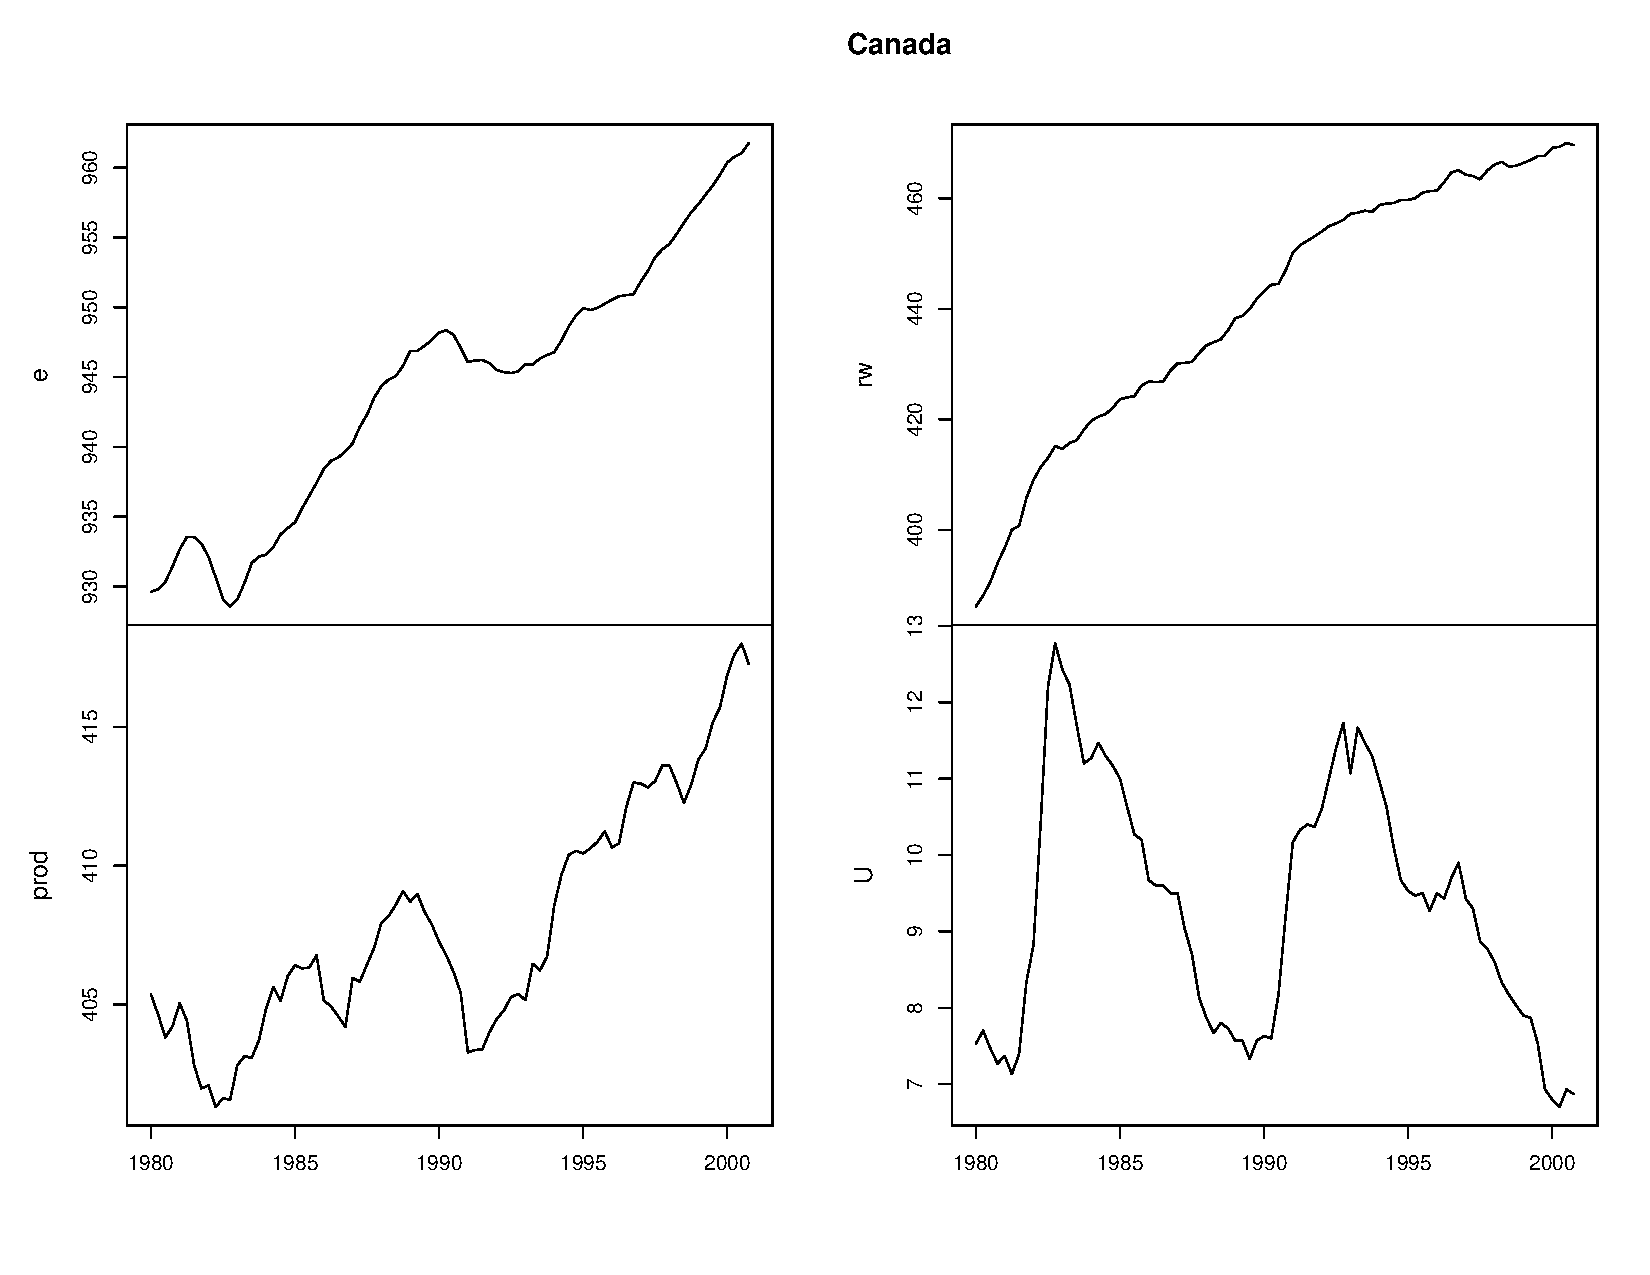
\includegraphics[width=\linewidth,scale=0.5]{canada.pdf}}
		\caption{e: logaritmo del empleo, prod: productividad definida como la log diferencia entre GDP y empleo,rw: salarios reales , U: tasa de desempleo.}\label{figd15}
%		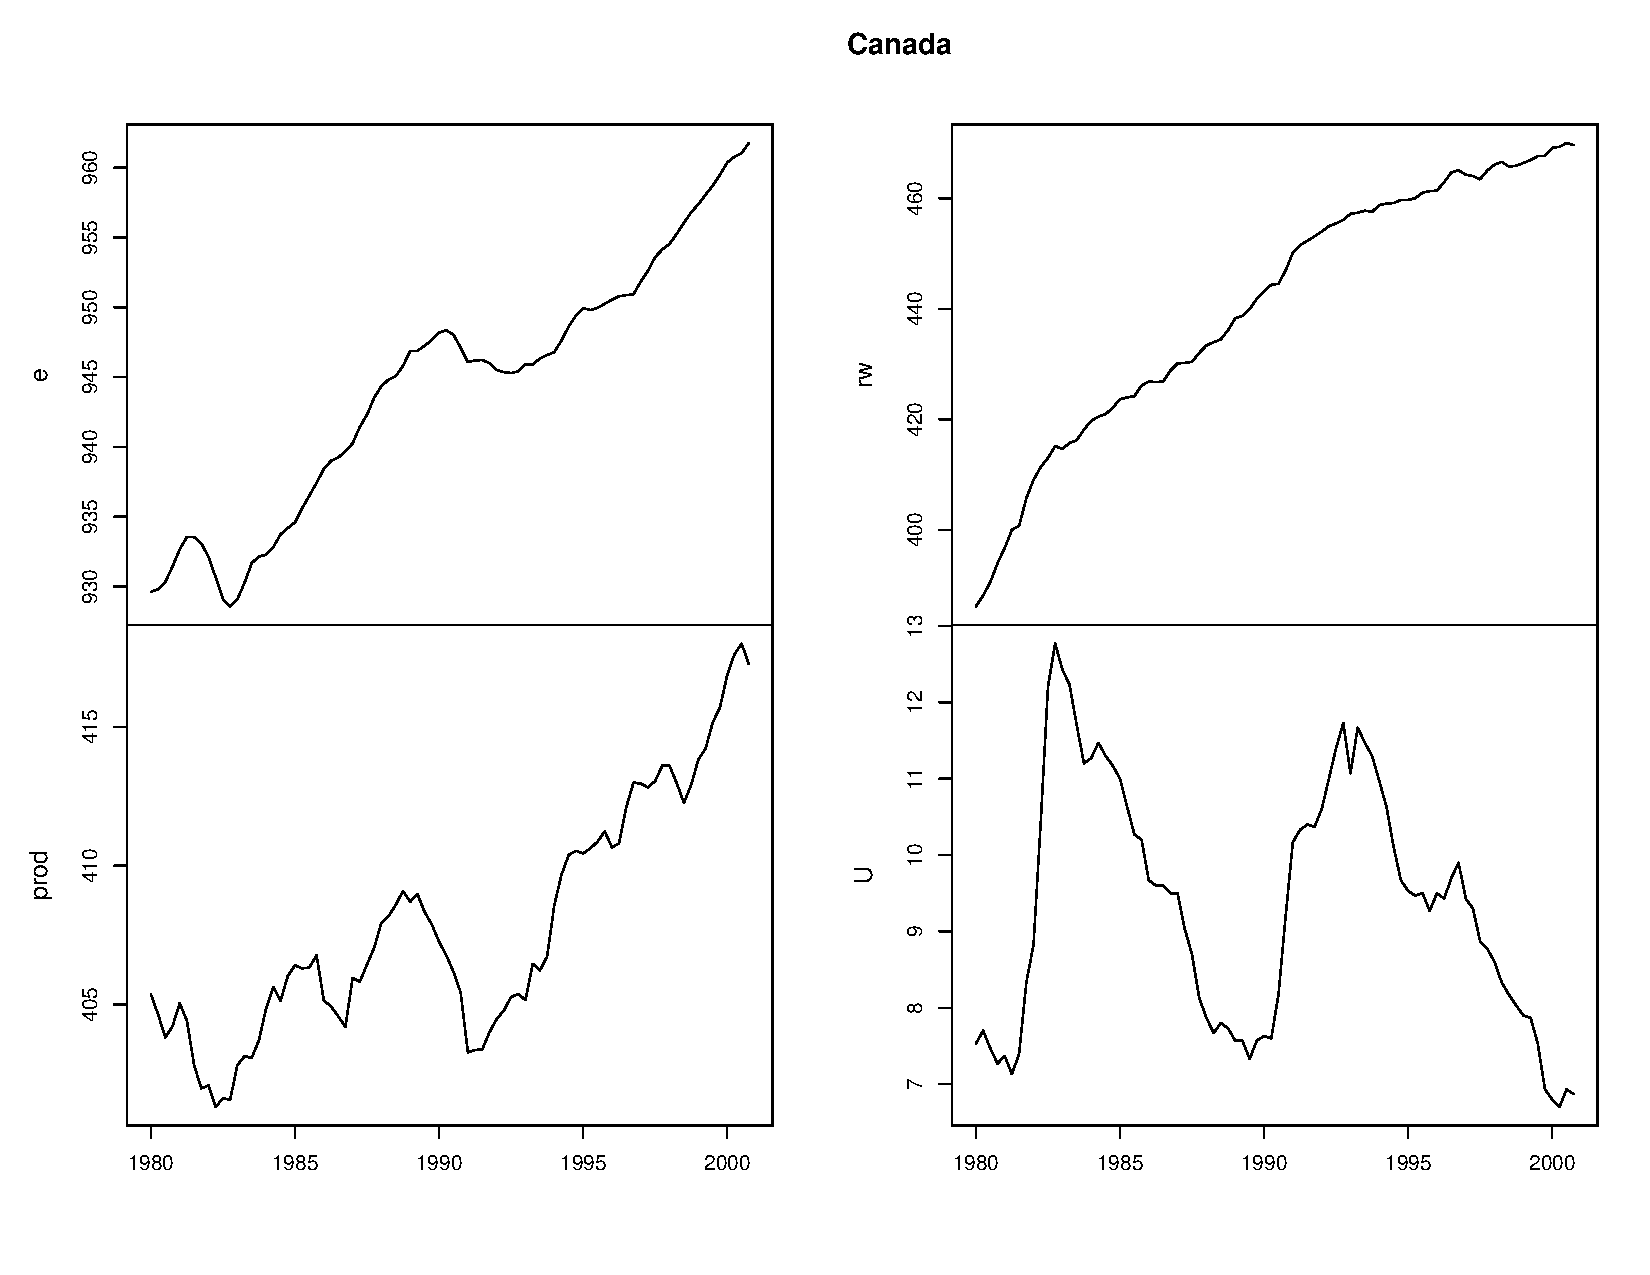
\includegraphics[scale=0.35]{canada.pdf}
	\end{figure}
	
%\end{frame}
%---------------------------------------------------------
%---------------------Slide 16--------------------------
%\begin{frame}
%	\frametitle{Vector Autoregressive Models}
%	\textbf{Ejemplo Modelo VAR}
	
	
	\begin{figure}[H]
		\centering
		\textbf{Modelo VAR: resumen de variables}\par\medskip
		\fcolorbox{green}{blue}{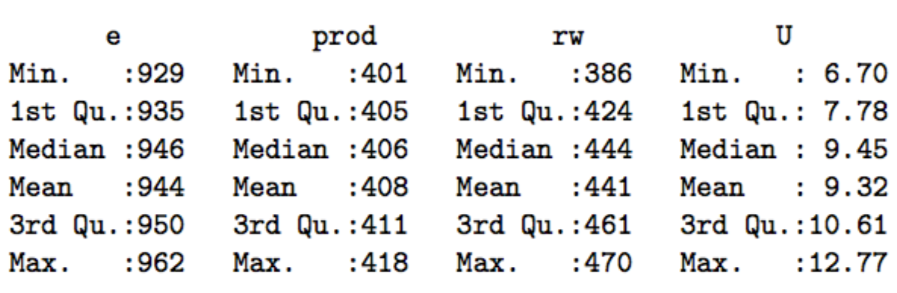
\includegraphics[width=\linewidth,scale=0.5]{summ.png}}
		\caption{Estadística resumen para variables del modelo VAR.}\label{figd16}
%		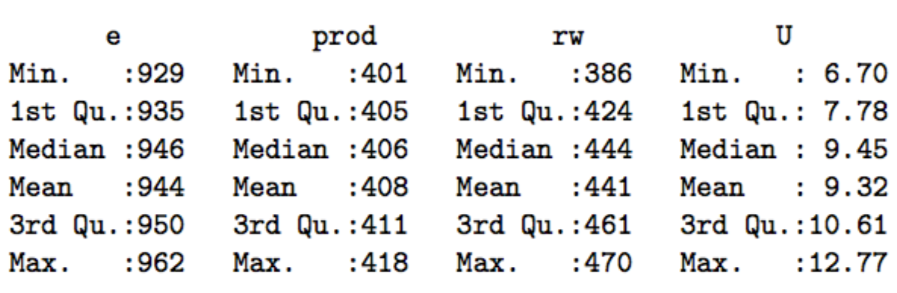
\includegraphics[scale=0.5]{summ.pdf}
	\end{figure}
	
%\end{frame}

%---------------------------------------------------------
%---------------------Slide 17--------------------------
%\begin{frame}
%	\frametitle{Vector Autoregressive Models}
%	\textbf{Ejemplo Modelo VAR}
	\begin{figure}[H]
		\centering
		\textbf{Ejemplo VAR: Augmented DF Test Unit Root Test}\par\medskip
		\fcolorbox{green}{blue}{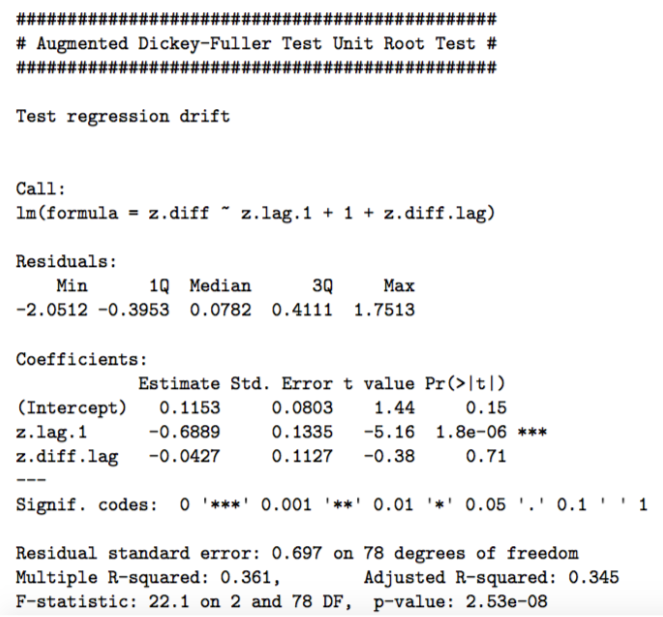
\includegraphics[scale=0.5]{df.png}}
		\caption{Test de Dickey-Füller Aumentado para evaluar la presencia de raiz unitaria en la serie  \textquotedblleft prod \textquotedblright. El modelo es considerado con \textquotedblleft drift \textquotedblright y un rezago(lags=1).}\label{figd17}
%		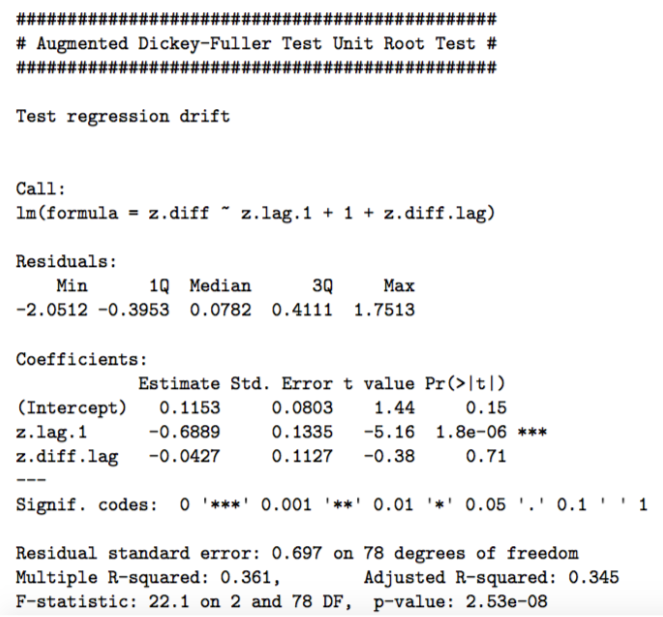
\includegraphics[scale=0.32]{df.pdf}
	\end{figure}
	
%\end{frame}

%---------------------------------------------------------
%---------------------Slide 18--------------------------
%\begin{frame}
%	\frametitle{Vector Autoregressive Models}
%	\textbf{Ejemplo Modelo VAR}
%	
%	\only<1|handout:1>{
%		\begin{exampleblock}{C\'odigo en R}
%			
%			VARselect(Canada, lag.max = 8, type = ``both")\\
%			Canada $<-$ Canada[, c(``prod", ``e", ``U", ``rw")]\\
%			p1ct $<-$ VAR(Canada, p = 1, type = ``both")\\
%			p1ct\\
%			\\
%			summary(p1ct, equation = ``e")\\
%			plot(p1ct, names = ``e")\\
%			\\
%			ser11 $<-$ serial.test(p1ct, lags.pt = 16, type = ``PT.asymptotic")\\
%			ser11$serial\\
%			\\
%			norm1 $<-$ normality.test(p1ct)\\
%			norm1$\$$jb.mul\\
%			\\
%			prd $<-$ predict(plct, n.ahead = 10, ci = 0.95, dumvar = NULL)\\
%			print(prd)\\
%			plot(prd, ``single")
%			
%		\end{exampleblock}
%	}
%	
%\end{frame}
\pagebreak
\lstset{caption=Ejemplo Modelo VAR2,framexleftmargin=5mm, frame=shadowbox, rulesepcolor=\color{green}}
\begin{lstlisting}[title={‘Código R: ejemplo Modelo VAR Mercado laboral canadiense},basicstyle=\ttfamily]{}
VARselect(Canada,lag.max = 8,type = "both")
Canada<Canada[, c("prod", "e", "U", "rw")]

p1ct<-VAR(Canada, p = 1, type = "both")
p1ct
summary(p1ct, equation = "e")
plot(p1ct, names = "e")

ser11<-serial.test(p1ct, lags.pt = 16, type = "PT.asymptotic")
ser11$serial
norm1<-normality.test(p1ct)
norm1$jb.mul
prd<-predict(p1ct, n.ahead = 10, ci = 0.95, dumvar = NULL)
print(prd)
plot(prd, "single")

\end{lstlisting}

%---------------------------------------------------------
%---------------------Slide 19--------------------------
%\begin{frame}
%	\frametitle{Vector Autoregressive Models}
%	\textbf{Ejemplo Modelo VAR - instrucci\'on VARselect}
	
	\begin{figure}[H]
		\centering
		\textbf{Ejemplo Modelo VAR: selección de modelos: instrucci\'on VARselect}\par\medskip
		\fcolorbox{green}{blue}{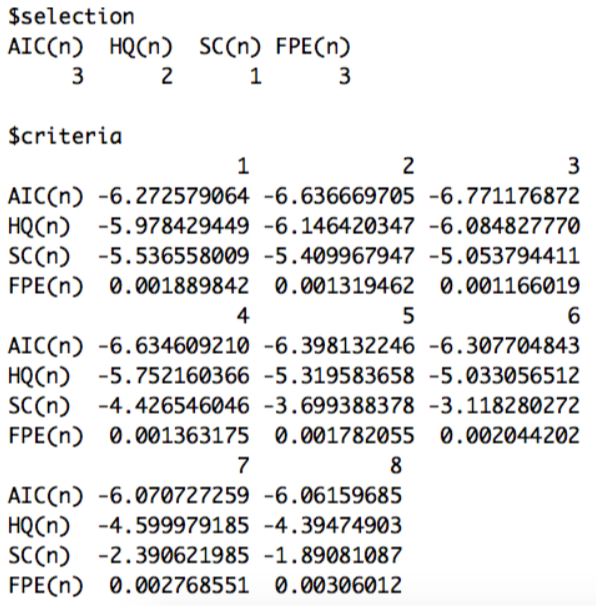
\includegraphics[scale=0.4]{selection.png}}
		\caption{Cada uno de los modelos contiene mediciones de AIC, HQ, SC y FPE}\label{fig34}
%		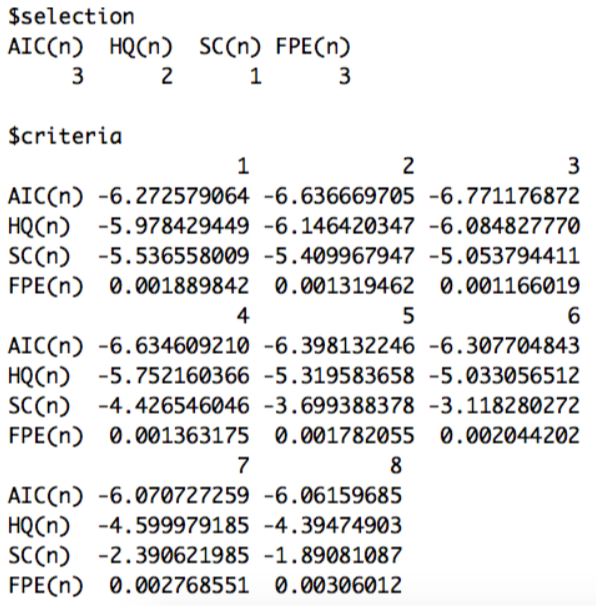
\includegraphics[scale=0.4]{selection.pdf}
	\end{figure}
	
%\end{frame}

%---------------------------------------------------------

%---------------------Slide 20--------------------------
%\begin{frame}
%	\frametitle{Vector Autoregressive Models}
%	\textbf{Ejemplo Modelo VAR - instrucci\'on VAR}
	
	\begin{figure}[H]
		\centering
		\textbf{Ejemplo Modelo VAR: instrucción VAR}\par\medskip
		\fcolorbox{green}{blue}{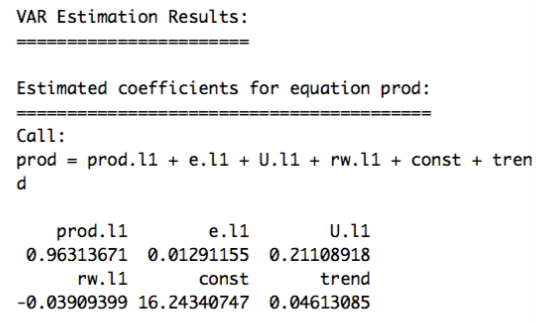
\includegraphics[width=\linewidth,scale=0.5]{var1.png}}
		\caption{Coeficientes de la ecuación pea variable \textquotedblleft prod \textquotedblright.}\label{fig35}
%		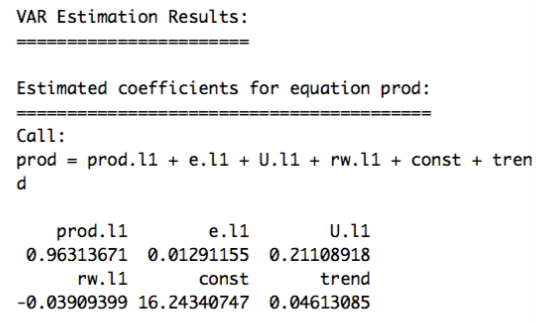
\includegraphics[scale=0.4]{var1.pdf}
	\end{figure}
	
		\begin{figure}[H]
		\centering
		\textbf{Ejemplo Modelo VAR: instrucción VAR}\par\medskip
		\fcolorbox{green}{blue}{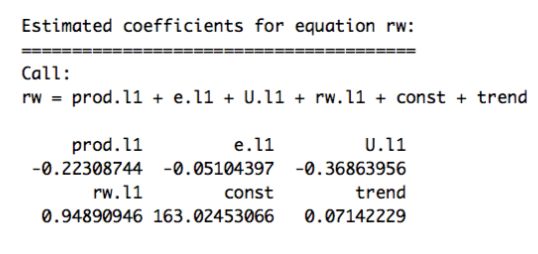
\includegraphics[width=\linewidth,scale=0.4]{var2.png}}
		\caption{Coeficientes de la ecuación pea variable \textquotedblleft rw \textquotedblright.}\label{fig36}
		%		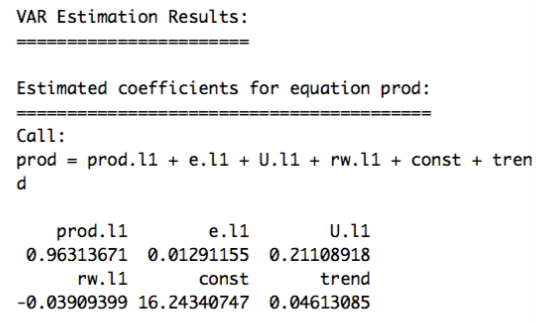
\includegraphics[scale=0.4]{var1.pdf}
	\end{figure}
		\begin{figure}[H]
		\centering
		\textbf{Ejemplo Modelo VAR: instrucción VAR}\par\medskip
		\fcolorbox{green}{blue}{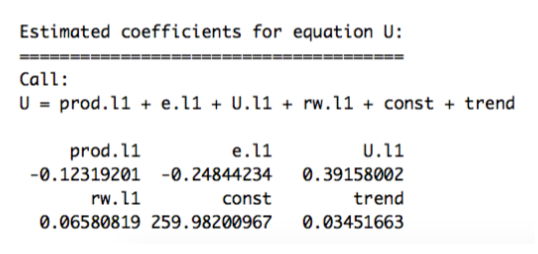
\includegraphics[width=\linewidth,scale=0.4]{var3.png}}
		\caption{Coeficientes de la ecuación pea variable \textquotedblleft U \textquotedblright.}\label{fig37}
		%		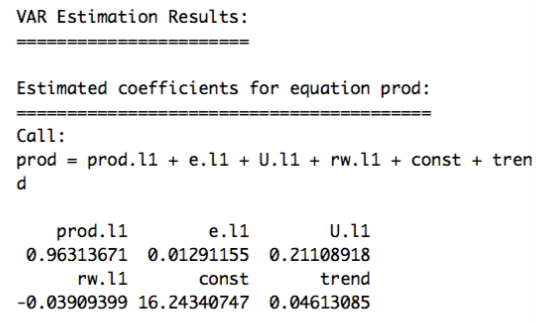
\includegraphics[scale=0.4]{var1.pdf}
	\end{figure}
		\begin{figure}[H]
		\centering
		\textbf{Ejemplo Modelo VAR: instrucción VAR}\par\medskip
		\fcolorbox{green}{blue}{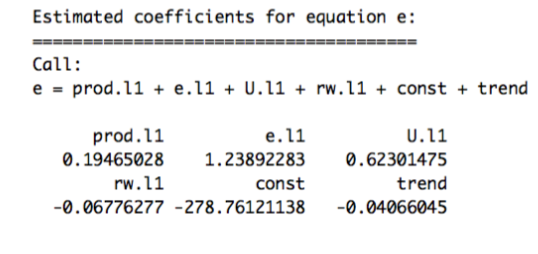
\includegraphics[width=\linewidth,scale=0.4]{var4.png}}
		\caption{Coeficientes de la ecuación para variable \textquotedblleft e \textquotedblright.}\label{fig38}
		%		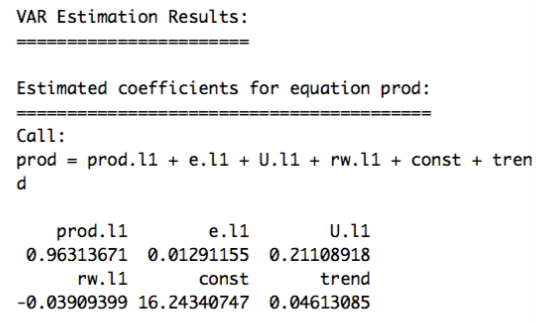
\includegraphics[scale=0.4]{var1.pdf}
	\end{figure}
%	
%%\end{frame}
%%---------------------------------------------------------
%%---------------------Slide 21--------------------------
%\begin{frame}
%	\frametitle{Vector Autoregressive Models}
%	\textbf{Ejemplo Modelo VAR - instrucci\'on VAR}
%	
%	\begin{figure}[t!]
%		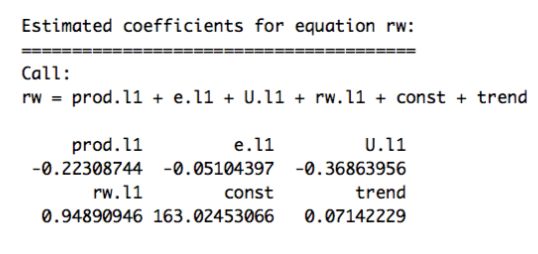
\includegraphics[scale=0.4]{var2.pdf}
%	\end{figure}
%	
%\end{frame}
%%---------------------------------------------------------
%%---------------------Slide 22--------------------------
%\begin{frame}
%	\frametitle{Vector Autoregressive Models}
%	\textbf{Ejemplo Modelo VAR - instrucci\'on VAR}
%	
%	\begin{figure}[t!]
%		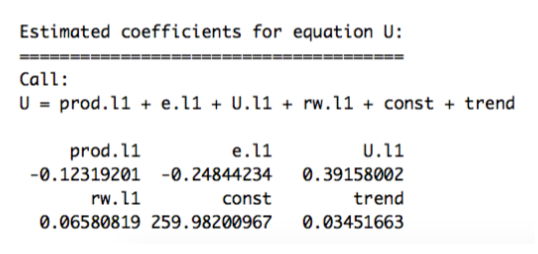
\includegraphics[scale=0.4]{var3.pdf}
%	\end{figure}
%	
%\end{frame}
%---------------------------------------------------------
%---------------------Slide 23--------------------------
%\begin{frame}
%	\frametitle{Vector Autoregressive Models}
%	\textbf{Ejemplo Modelo VAR - instrucci\'on VAR para e}
	
	\begin{figure}[H]\label{figd23}
		\centering
		\textbf{Ejemplo Modelo VAR - instrucci\'on VAR para e}\par\medskip
		\fcolorbox{green}{blue}{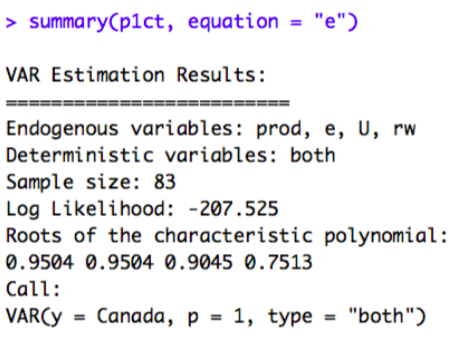
\includegraphics[width=\linewidth,scale=0.4]{var-e1.png}}
%		\caption{}
%		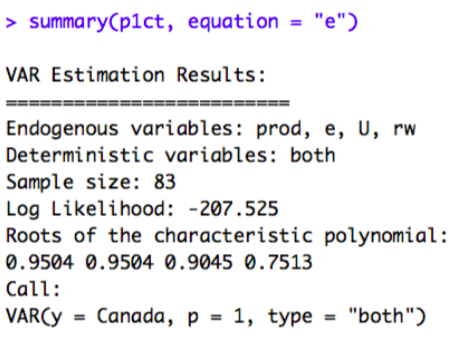
\includegraphics[scale=0.45]{var-e1.png}
	\end{figure}
	
%\end{frame}
%---------------------------------------------------------
%---------------------Slide 24--------------------------
%\begin{frame}
%	\frametitle{Vector Autoregressive Models}
%	\textbf{Ejemplo Modelo VAR - instrucci\'on VAR para e}
	
	\begin{figure}[H]
		\centering
		\textbf{Ejemplo Modelo VAR - instrucci\'on VAR para e}\par\medskip
		\fcolorbox{green}{blue}{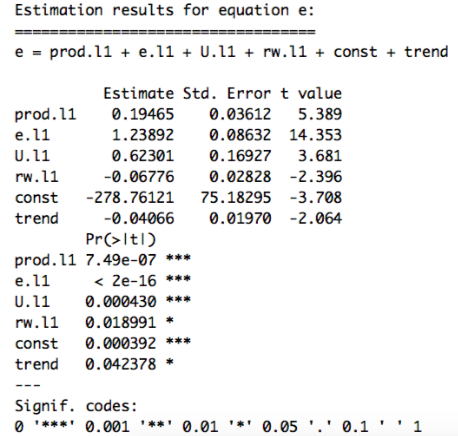
\includegraphics[width=\linewidth,scale=0.5]{var-e2.png}}
		\caption{Evaluación de los parámetros en la ecuación del VAR para variable \textquotedblleft e\textquotedblright.}\label{figd24}
%		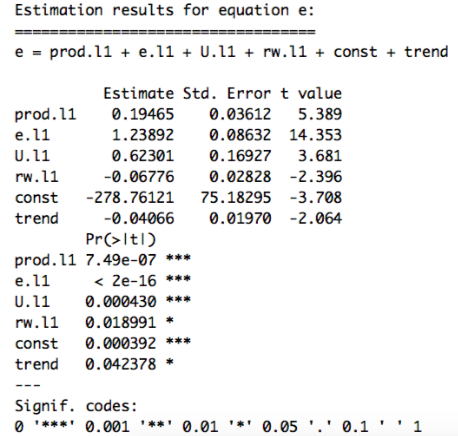
\includegraphics[scale=0.35]{var-e2.png}
	\end{figure}
	
%\end{frame}
%---------------------------------------------------------
%---------------------Slide 25--------------------------
%\begin{frame}
%	\frametitle{Vector Autoregressive Models}
%	\textbf{Ejemplo Modelo VAR - instrucci\'on VAR para e}
	
\begin{figure}[H]
		\centering
		\textbf{Ejemplo Modelo VAR - instrucci\'on VAR para e}\par\medskip
		\fcolorbox{green}{blue}{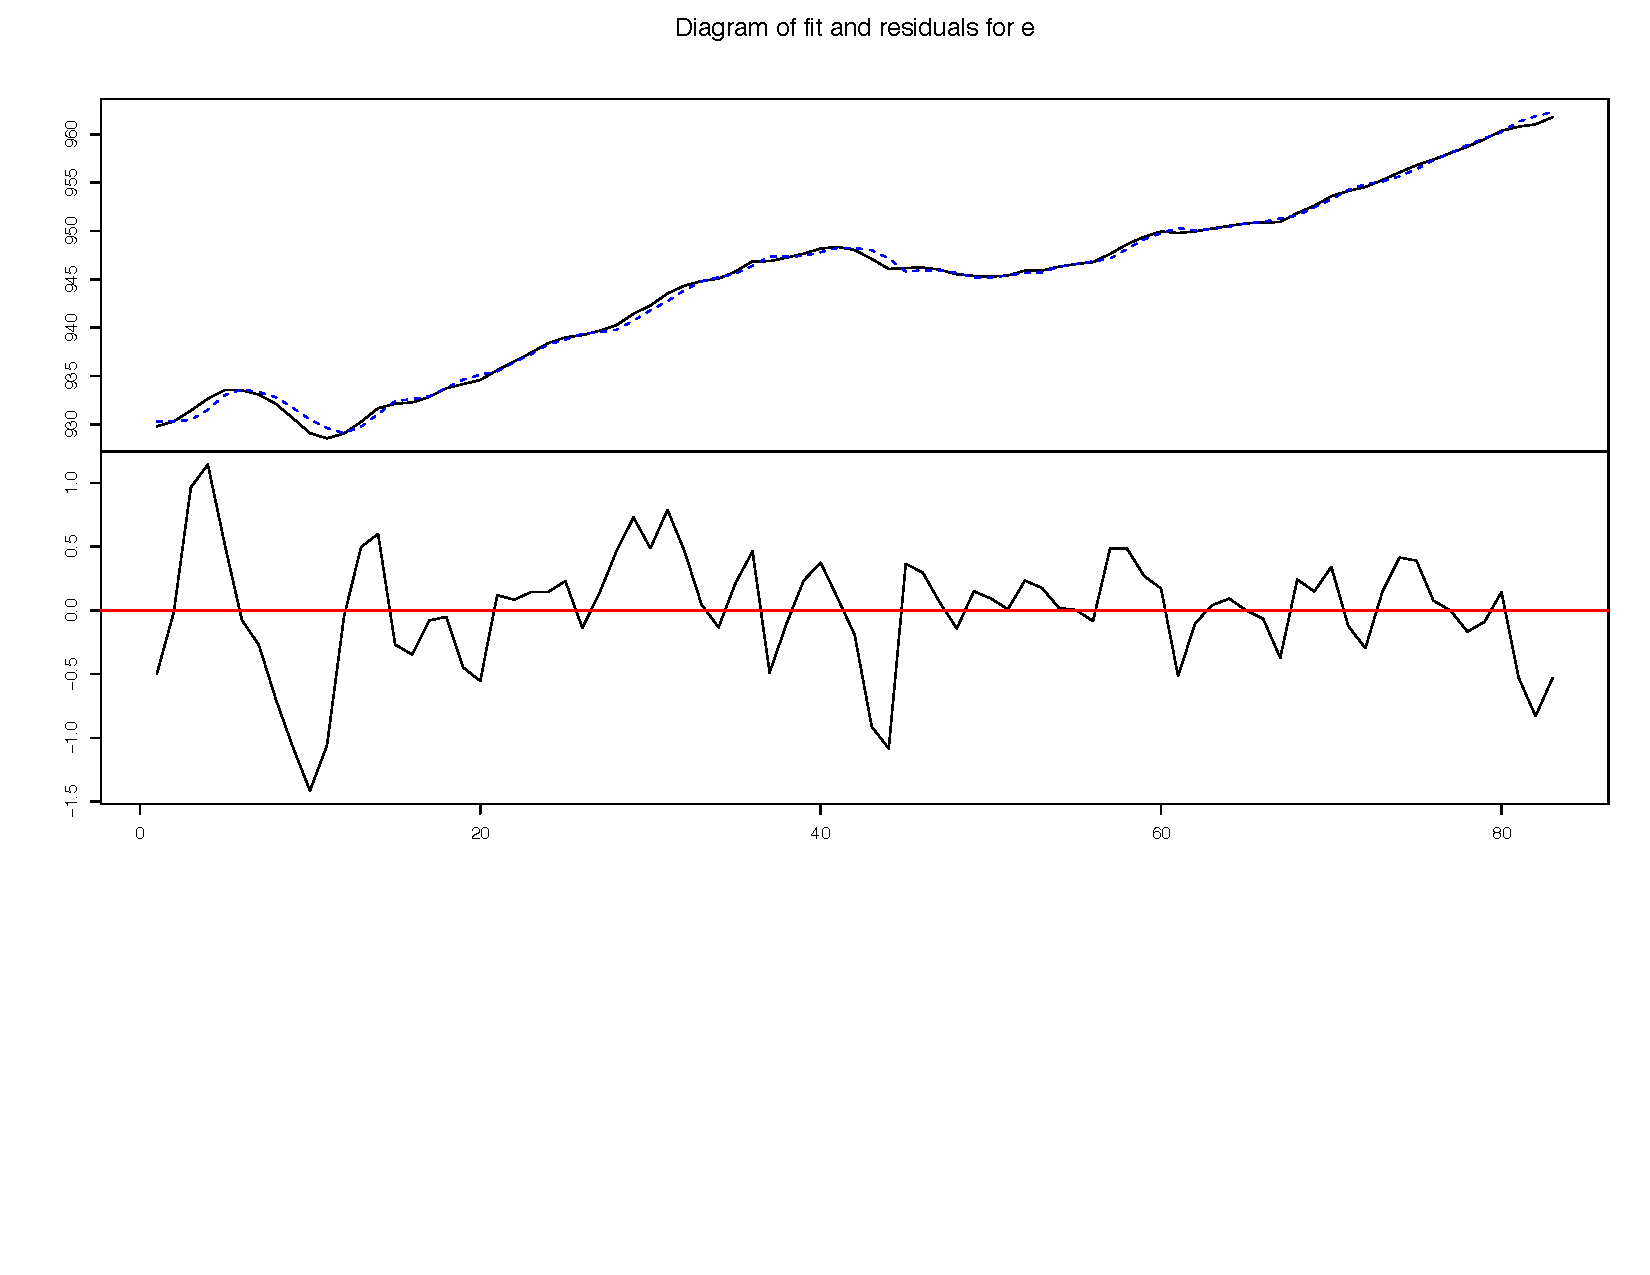
\includegraphics[width=\linewidth,scale=0.5]{var_fig.pdf}}
		\caption{Diagrama del ajuste de residuos para ecuación  \textquotedblleft e \textquotedblright.}\label{fig52}
%		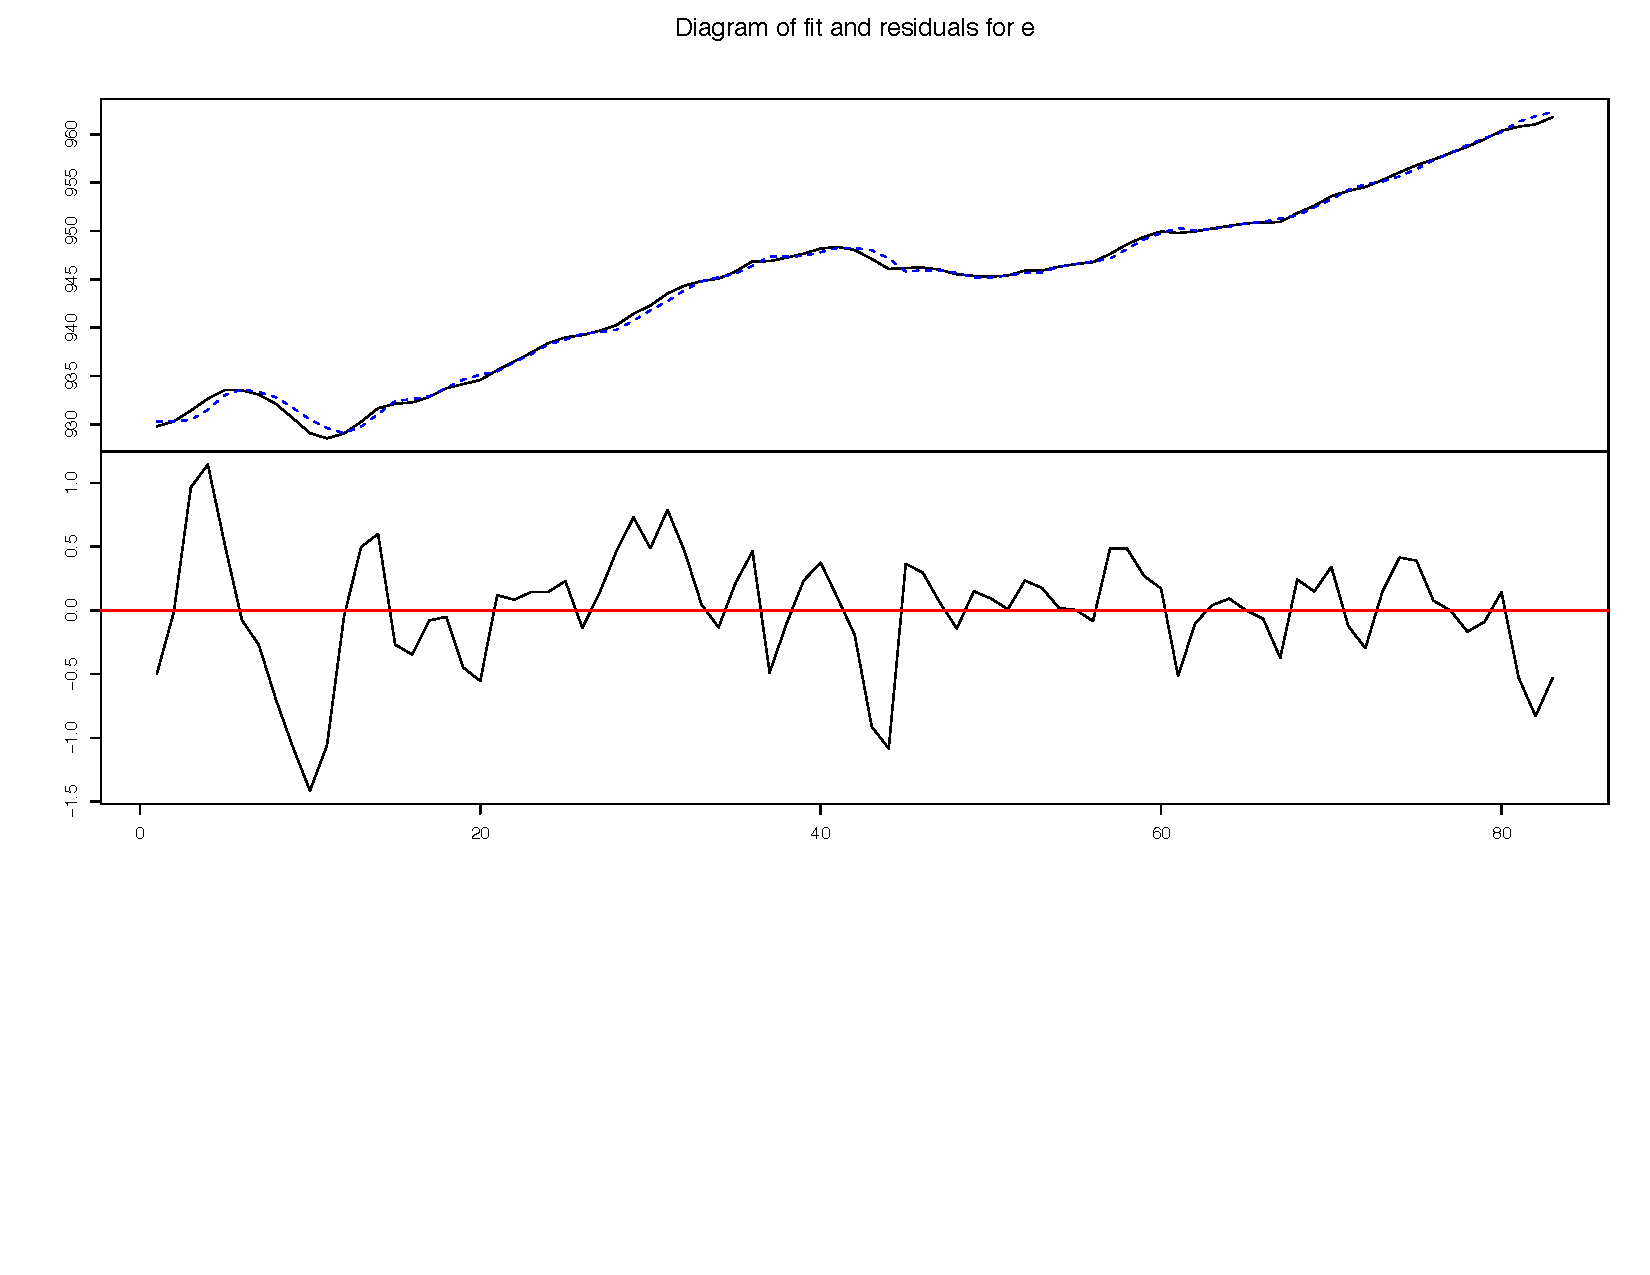
\includegraphics[scale=0.35]{var_fig.pdf}
\end{figure}
	
%\end{frame}
%---------------------------------------------------------
%---------------------Slide 26--------------------------
%\begin{frame}
%	\frametitle{Vector Autoregressive Models}
%	\textbf{Ejemplo Modelo VAR - instrucci\'on VAR para e}
	
	\begin{figure}[H]\label{figd26}
		\centering
		\textbf{Ejemplo Modelo VAR - instrucci\'on VAR para e}\par\medskip
		\fcolorbox{green}{blue}{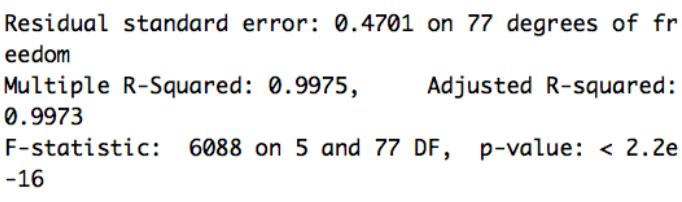
\includegraphics[width=\linewidth,scale=0.5]{var-e3.png}}
%		\caption{Colocar nota explicativa de figura}
%		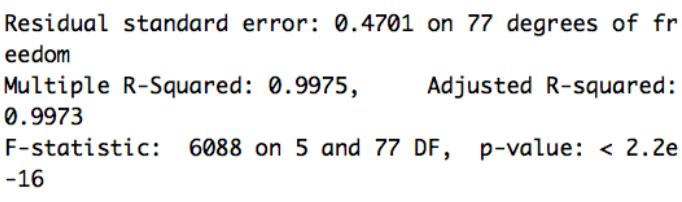
\includegraphics[scale=0.45]{var-e3.png}
	\end{figure}
	
%\end{frame}
%---------------------------------------------------------
%---------------------Slide 27--------------------------
%\begin{frame}
%	\frametitle{Vector Autoregressive Models}
%	\textbf{Ejemplo Modelo VAR - instrucci\'on VAR para e}
	
	\begin{figure}[H]
		\centering
		\textbf{Ejemplo Modelo VAR - instrucci\'on VAR para e}\par\medskip
		\fcolorbox{green}{blue}{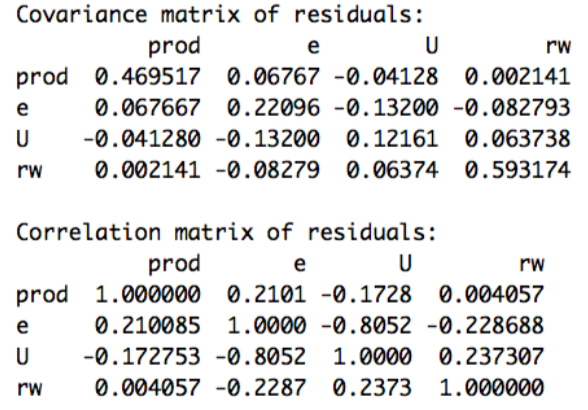
\includegraphics[width=\linewidth,scale=0.5]{var-e4.png}}
		\caption{Matriz de covarianza y de correlación de modelo VAR}\label{fig44}
%		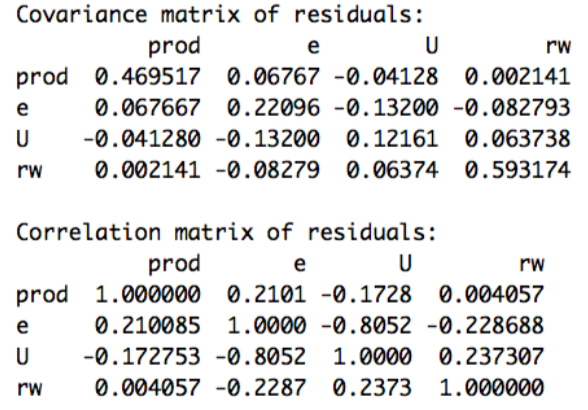
\includegraphics[scale=0.45]{var-e4.png}
	\end{figure}
	
%\end{frame}
%\end{section}
%---------------------------------------------------------
%---------------------Slide 28--------------------------
%\begin{frame}
%\frametitle{Vector Autoregressive Models}
%\textbf{Ejemplo Modelo VAR - instrucci\'on VAR para e}

\begin{figure}[H]
	\centering
	\textbf{Ejemplo Modelo VAR - instrucci\'on VAR para \textquotedblleft e\textquotedblright}\par\medskip
	\fcolorbox{green}{blue}{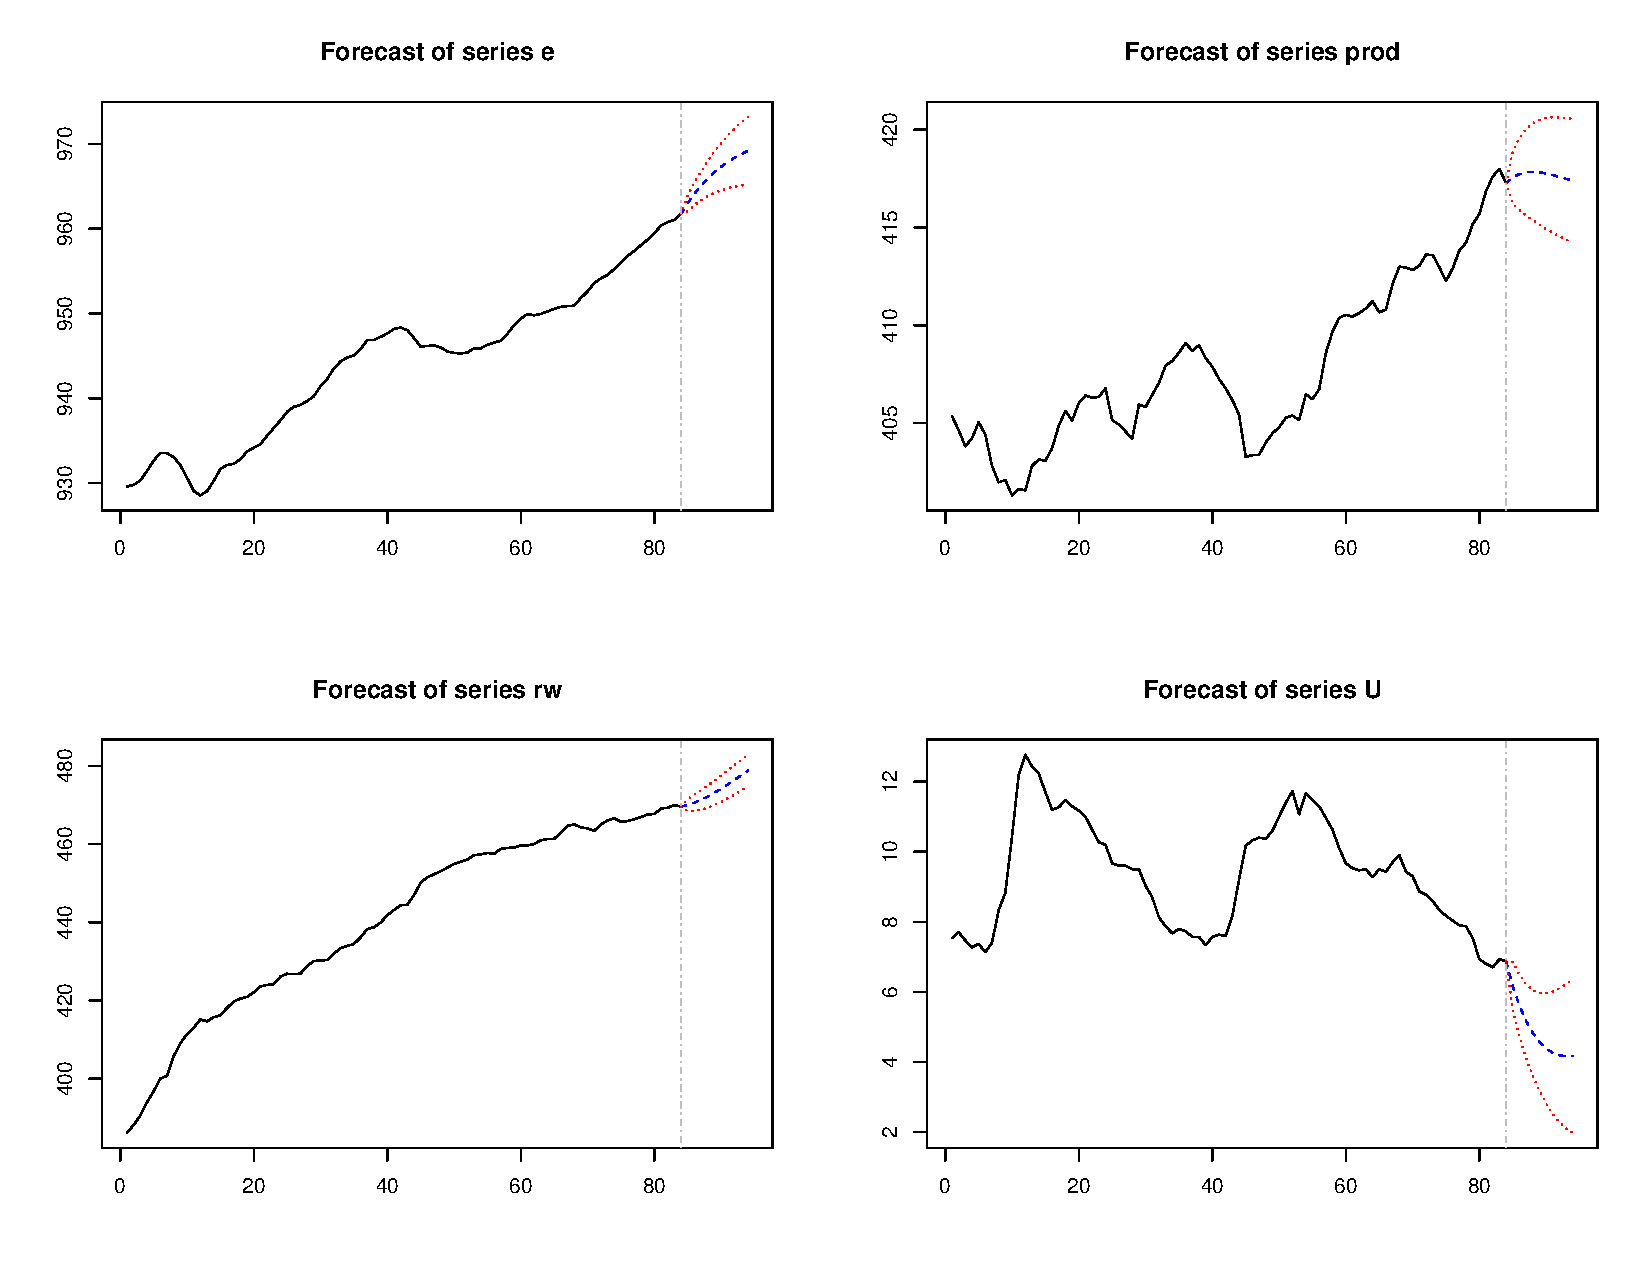
\includegraphics[scale=0.6]{forecastVAR.pdf}}
	\caption{Pronosticos de modelo VAR.}\label{fig45}
%	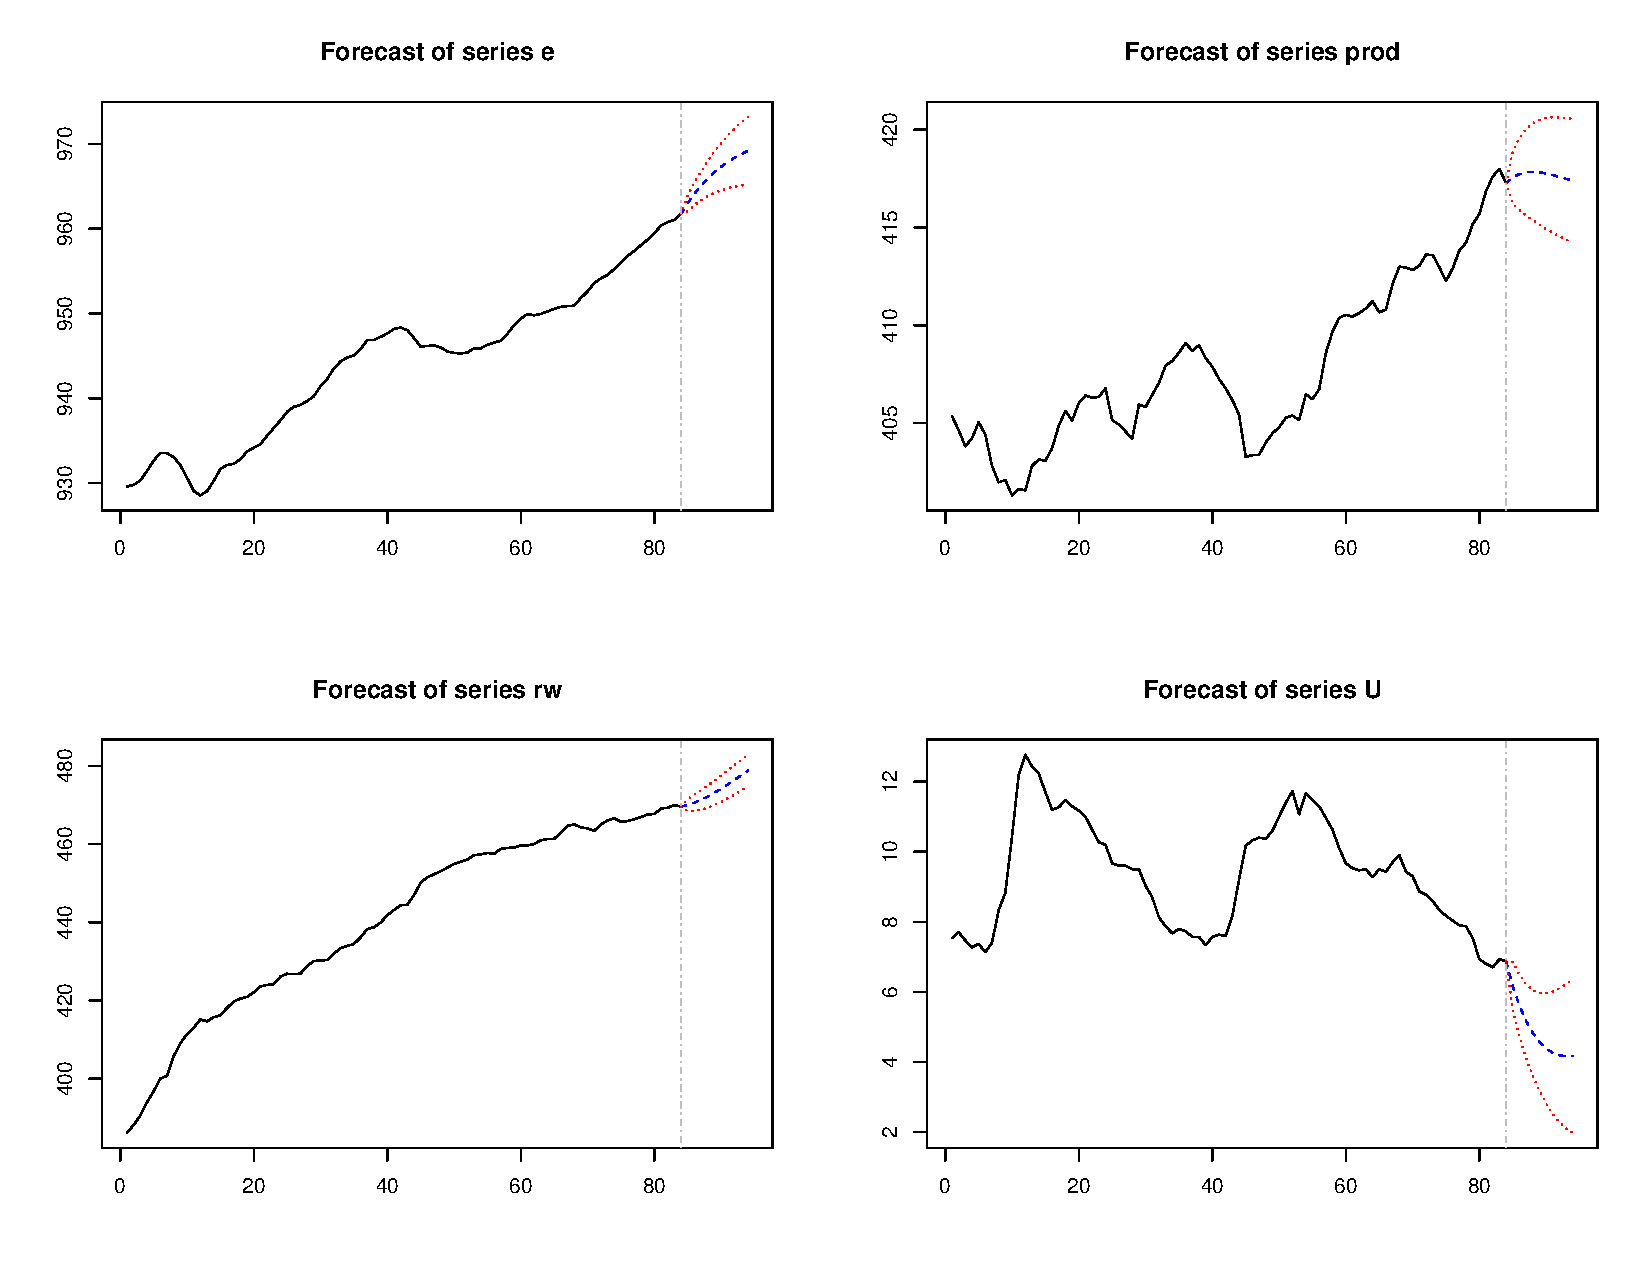
\includegraphics[scale=0.25]{forecastVAR.pdf}
\end{figure}

%\end{frame}
%---------------------------------------------------------
%---------------------Slide 29--------------------------
%\begin{section}{Forma Primitiva versus Forma Estándar de VARs}
%\begin{frame}
%	\frametitle{Vector Autoregressive Models}
\pagebreak\subsection{Forma Primitiva versus Forma Estándar de VARs}	
	\textbf{?`Incluye el modelo VAR t\'erminos contempor\'aneos?}
	Hasta el momento, hemos asumido que el modelo VAR es de la forma:\\
	\begin{equation*}
	y_{1t} = \beta_{10} + \beta_{11} y_{1t-1} + \alpha_{11} y_{2t-1} + \mu_1t
	\end{equation*}
	\begin{equation*}
	y_{2t} = \beta_{20} + \beta_{21} y_{2t-1} + \alpha_{21} y_{1t-1} + \mu_2t
	\end{equation*}
	Pero, ?`qu\'e pasa si las ecuaciones ten\'{i}an un t\'ermino retroalimentaci\'on contempor\'aneo?\\
	\begin{equation*}
	y_{1t} = \beta_{10} + \beta_{11} y_{1t-1} + \alpha_{11} y_{2t-1} + \alpha_{12} y_{2t} + \mu_1t
	\end{equation*}
	\begin{equation*}
	y_{2t} = \beta_{20} + \beta_{21} y_{2t-1} + \alpha_{21} y_{1t-1} + \alpha_{22} y_{1t} + \mu_2t
	\end{equation*}

%\end{frame}
%---------------------------------------------------------
%---------------------Slide 30--------------------------
%\begin{frame}
%	\frametitle{Vector Autoregressive Models}	
	Podemos escribir esto como:\\
	\begin{gather*}
	\begin{pmatrix} y_{1t} \\ y_{2t} \end{pmatrix}
	=
	\begin{pmatrix} \beta_{10} \\ \beta_{20} \end{pmatrix}
	+
	\begin{pmatrix} \beta_{11} & \alpha_{11} \\ \alpha_{21} & \beta_{21} \end{pmatrix}
	\begin{pmatrix} y_{1t-1} \\ y_{2t-1} \end{pmatrix}
	+
	\begin{pmatrix} \alpha_{12} & 0 \\ 0 & \alpha_{22} \end{pmatrix}
	\begin{pmatrix} y_{1t-1} \\ y_{2t-1} \end{pmatrix}
	+
	\begin{pmatrix} \mu_{1t} \\ \mu_{2t} \end{pmatrix}
	\end{gather*}
	Este VAR est\'a en su forma primitiva….
	
%\end{frame}
%---------------------------------------------------------
%---------------------Slide 31--------------------------
%\begin{frame}
%	\frametitle{Vector Autoregressive Models}
%	
	\textbf{Forma Primitiva versus Forma Estándar de VARs}
	
	Podemos tomar los t\'erminos contempor\'aneos del LHS (lado izquierdo) y escribir:
	\begin{gather*}
	\begin{pmatrix} 1 & -\alpha_{12} \\ -\alpha_{22} & 1 \end{pmatrix}
	\begin{pmatrix} y_{1t} \\ y_{2t} \end{pmatrix}
	=
	\begin{pmatrix} \beta_{10} \\ \beta_{20} \end{pmatrix}
	+
	\begin{pmatrix} \beta_{11} & \alpha_{11} \\ \alpha_{21} & \beta_{21} \end{pmatrix}
	\begin{pmatrix} y_{1t-1} \\ y_{2t-1} \end{pmatrix}
	+
	\begin{pmatrix} \mu_{1t} \\ \mu_{2t} \end{pmatrix}
	\end{gather*}
	
	\'o
	\begin{equation*}
	By_{t} = \beta_{0} + \beta_{1} y_{t-1} + \mu_t
	\end{equation*}
	
	Podemos entonces multiplicar ambos lados por $B^-1$ y obtener:
	\begin{equation*}
	y_{t} = B^-1\beta_{0} + B^-1\beta_{1} y_{t-1} + B^-1\mu_t
	\end{equation*}
	\'o
	\begin{equation*}
	y_{t} = A_{0} + A_{1} y_{t-1} + e_t
	\end{equation*}
	Esto se conoce como un VAR en su Forma Est\'andar, y se puede estimar por MCO.
	
%\end{frame}
%\end{section}
%%---------------------------------------------------------
%%---------------------Slide 32--------------------------
%\begin{section}{Estabilidad de los procesos VAR}
%\begin{frame}
%	\frametitle{Vector Autoregressive Models}
\pagebreak\subsection{Estabilidad de los procesos VAR}
	
%	\textbf{Estabilidad de los procesos VAR}
	
	Una caracter\'{i}stica importante de un proceso VAR (p) es su estabilidad. Esto significa que genera series de tiempo estacionarias con medias, varianzas y covarianzas  invariantes en el tiempo, dados suficientes valores iniciales. Uno puede verificar esto evaluando el polinomio caracter\'{i}stico:
	\begin{equation}
		det(I_K - A_{1z} - \dots{} - A_{p}z^p)=0.
	\end{equation}
	Para $|z|\le1$.\\
	Si la soluci\'on de la ecuaci\'on anterior tiene una ra\'{i}z para z = 1, entonces algunas o todas las variables en el proceso VAR (p) son integradas de la orden uno, es decir, I (1).\\
	
%\end{frame}
%%---------------------------------------------------------
%%---------------------Slide 33--------------------------
%\begin{frame}
%	\frametitle{Vector Autoregressive Models}
	
%	\textbf{Estabilidad de los procesos VAR}
	
	En la pr\'actica, la estabilidad de un proceso emp\'{i}rico de VAR (p) puede analizarse considerando la forma complementaria y calculando los valores propios de la matriz de coeficientes. Un proceso VAR (p) puede escribirse como un proceso VAR (1):
	\begin{equation*}
	\xi_t=A\xi_{t-1}+\nu_t
	\end{equation*}
	
	\begin{gather*}
	\xi_t=\begin{bmatrix} y_{t} \\ \vdots{} \\ y_{t-p+1} \end{bmatrix}
	,
	A=\begin{bmatrix} A_{1} & A_{2} & \dots{} & A_{p-1} & A_{p} \\
	I & 0 & \dots{} & 0 & 0 \\
	0 & I & \dots{} & 0 & 0 \\
	\vdots{} & \vdots{} & \ddots{} & \vdots{} & \vdots{} \\
	0 & 0 & \dots{} & I & 0 
	\end{bmatrix}
	,
	\nu_t=\begin{pmatrix} \mu_{t} \\ 0 \\ \vdots{} \\ 0 \end{pmatrix}
	\end{gather*}
	
	Las dimensiones de los vectores $\xi_t$ y $\nu_t$ son (KP × 1) y la dimensión de la matriz A es (Kp × Kp). Nuevamente, si los m\'odulos de los autovalores de A son menores que uno, entonces el proceso VAR (p) es estable.
	
%\end{frame}
%%---------------------------------------------------------
%%---------------------Slide 34--------------------------
%\begin{frame}
%	\frametitle{Vector Autoregressive Models}
	
%	\textbf{Estabilidad de los procesos VAR}
	
	Una muestra dada de las variables end\'ogenas $y_1,\dots{}, y_T$, y suficientes valores de muestra previa $y_{-p + 1},\dots{}, y_0$, los coeficientes de un proceso VAR (p) pueden estimarse eficientemente mediante m\'{i}nimos cuadrados aplicados por separado a cada una de las ecuaciones.\\
	
	Una vez que se ha estimado un modelo VAR (p), la avenida est\'a abierta para su posterior an\'alisis. Un investigador podr\'{i}a / deber\'{i}a estar interesado en las pruebas de diagn\'ostico, como las pruebas de ausencia de autocorrelaci\'on, heterocedasticidad o no normalidad en el t\'ermino de error.\\
	\'El podr\'{i}a estar m\'as interesado en la inferencia causal, el pron\'ostico y / o el diagn\'ostico del comportamiento din\'amico del modelo emp\'{i}rico, es decir, las funciones de respuesta al impulso (en adelante, IRF, por su sigla en ingl\'es \textbf{impulse response functions} y pronosticar la descomposición de la varianza del error (en lo sucesivo: FEVD, por su sigla en ingl\'es \textbf{forecast error variance decomposition }). \\
	
%\end{frame}
%%-------------------de-------------------------------------
%%---------------------Slide 35--------------------------
%\begin{frame}
%	\frametitle{Vector Autoregressive Models}
	Los dos \'ultimos se basan en la descomposici\'on media m\'ovil de Wold para procesos estables de VAR (p) que se define como:.
	\begin{equation*}
	y_t = \Phi_0u_t + \Phi_1u_{t-1} + \Phi_2u_{t-2} + \dots{}
	\end{equation*}
	
	con $\Phi_0 = I_K$ y $\Phi_s$ se pueden calcular recursivamente según: 
	\begin{equation*}
	\Phi_s = \sum_{j=1}^{s}\Phi_{s-j}A_j 
	\end{equation*}
	para $s = 1,2, \dots{}$ donde $A_j = 0$ para $j > p$.\\
	
%\end{frame}
%---------------------------------------------------------
%---------------------Slide 36--------------------------
%\begin{frame}
%	\frametitle{Vector Autoregressive Models}
	
	Finalmente, las predicciones para horizontes $h \le 1$ de un proceso emp\'{i}rico VAR (p) pueden generarse recursivamente seg\'un:
	\begin{equation*}
	y_{T + h | T} = A_1y_{T + h-1 | T} + \dots{} + A_py_{T + h-p | T} 
	\end{equation*}
	donde $y_{T + j | T} = y_{T + j}$ para $j \le 0$. 
%\end{frame}
%%---------------------------------------------------------
%%---------------------Slide 37--------------------------
%\begin{frame}
%	\frametitle{Vector Autoregressive Models}
	La matriz de covarianza de error de pron\'ostico es dado como:\\
	\footnotesize
	\begin{gather*}
	Cov\begin{bmatrix} y_{T + 1} - y_{T + 1 | T} \\ \vdots{} \\ y_{T + h} - y_{T + h | T} \end{bmatrix}
	=
	\begin{bmatrix} I & 0 & \dots{} & 0 \\
	\Phi_1 & I & \dots{}  & 0 \\
	\vdots{} & \vdots{} & \ddots{} &  0 \\
	\Phi_{h-1} & \Phi_{h-2} & \dots{} & I 
	\end{bmatrix}
	(\sum_u \otimes I_h)
	\begin{bmatrix} I & 0 & \dots{} & 0 \\
	\Phi_1 & I & \dots{}  & 0 \\
	\vdots{} & \vdots{} & \ddots{} &  0 \\
	\Phi_{h-1} & \Phi_{h-2} & \dots{} & I 
	\end{bmatrix}^T
	\end{gather*}
	
	y las matrices $\Phi_i$ son las matrices de coeficientes emp\'{i}ricos de la representaci\'on de media m\'ovil de Wold de un proceso VAR (p) estable como se muestra arriba. El operador $\otimes$ es el producto Kronecker.
	
%\end{frame}
%\end{section}
%%---------------------------------------------------------
%%---------------------Slide 38--------------------------
%\begin{section}{Las respuestas de impulso y descomposiciones de la varianza}
%\begin{frame}
%	\frametitle{Vector Autoregressive Models}
\subsection{Las respuestas de impulso y descomposiciones de la varianza}
	
	\textbf{Ejemplo Impulse Responses - funci\'on de respuesta al impulso}\\
	Los modelos VAR son a menudo dif\'{i}ciles de interpretar. Soluciones a este problema, como vimos, son la construcci\'on de funciones de respuestas a impulso y las descomposiciones de la varianza.
	
	Las funciones de respuesta al impulso muestran la capacidad de respuesta de las variables dependientes en el VAR a shocks al t\'ermino de error. Una unidad de shock se aplica a cada variable y sus efectos son almacenados.
	
%\end{frame}
%---------------------Slide 39--------------------------
%\begin{frame}
%	\frametitle{Vector Autoregressive Models}
	
%	\textbf{Ejemplo Impulse Responses - funci\'on de respuesta al impulso}\\
	
	Considere, por ejemplo, un VAR(1) bivariante sencillo:
	
	\begin{equation*}
	y_{1t} = \beta_{10} + \beta_{11} y_{1t-1} + \alpha_{11} y_{2t-1} + \mu_{1t}
	\end{equation*}
	\begin{equation*}
	y_{2t} = \beta_{20} + \beta_{21} y_{2t-1} + \alpha_{21} y_{1t-1} + \mu_{2t}
	\end{equation*}
Inicialmente, en $t=1$ suponemos un shock en el término de error $\mu_{11}$ de la primera ecuación. Este impacto tiene un efecto directo en $y_{11}$, de exactamente la misma cantidad.
Considerando que $y_{21}$ todavía no se efectúa, y suponiendo que $\mu_{21}=0$ con $t=1, \dots T$. En el segundo período (t=2), el impacto original todavía tiene un efecto sobre el valor rezagado de $y_{1}$. El efecto en $y_{12}$, es $\beta_{11}\mu_{11}$, y el efecto en $y_{22}$ es $\beta_{21}\mu_{11}$. En el tercer período, el efecto sobre $y_{13}$, no es solo $\beta_{11}(\beta_{11}\mu_{11})$, sino también $\beta{12}(\beta{21}\mu{11})$. En consecuencia, el efecto sobre $y_{23}$ es $\beta_{21}(\beta_{21}\mu_{11})+\beta{22}(\beta_{21}\mu_{11})$.

%En el tercer per\'{i}odo, el efecto sobre $y_{13}$, 􏰞no es solo 􏰁􏰁$\beta_{11}(\beta_{11}\mu_{11})$􏰁􏰁, sino también 􏰁􏰁$\beta_{12}(\beta_{21}\mu_{11})$􏰁􏰆􏰗􏰆􏰁􏰁􏰘. En consecuencia, el efecto sobre $y_{23}$ 􏰞 es 􏰁􏰁$\beta_{21}(\beta_{21}\mu_{11})+\beta_{22}(\beta_{21}\mu_{11})$􏰁􏰁􏰆􏰁􏰗􏰆􏰁􏰁􏰁􏰘􏰆􏰆􏰗􏰆􏰆􏰗􏰆􏰁􏰁. 	
%\end{frame}
%---------------------------------------------------------
%\begin{frame}
%	\frametitle{Vector Autoregressive Models}
	
%\textbf{Ejemplo Impulse Responses - funci\'on de respuesta al impulso}\\
Por lo tanto, es posible resumir el efecto de un shock no recurrente en una variable, con todas las variables a lo largo del tiempo. Uno podr\'{i}a resumir el resultado anterior en:
\begin{equation}
y_t = \sum_{k=0}^{\infty}  C_k \mu_{t-k}
\end{equation}
%	donde como vimos, $C􏰝_0= I$ (Vector-Moving-Average Process) y donde $C􏰟_k$ son el peso de las existencias anteriores.
donde como vimos, $C_{0}=I$ (Vector-Moving-Average Process) y donde $C_{k}$ son el peso de las existencias anteriores. 	
%\end{frame}

%---------------------------------------------------------
%---------------------Slide 41--------------------------
%\begin{frame}
%	\frametitle{Vector Autoregressive Models}
	
	\textbf{Ejemplo Orthogonal Impulse Responses}\\
	
	En el modelo anterior de respuesta al impulso, asumimos que los t\'erminos de error de la ecuaci\'on diferente no est\'an correlacionados. Sin embargo, esta suposici\'on es bastante poco plausible. Un choque hipot\'etico en una sola ecuaci\'on no responde a un proceso de ajuste realista. Para controlar la correlaci\'on entre los t\'erminos de error, tenemos que usar las secuencias de respuesta de impulso ortogonal. La idea es modificar la construcci\'on media m\'ovil original de forma que los residuos no est\'en correlacionados, es decir, los residuos deben ser ortogonales entre si. Por lo tanto, podemos escribir:
	\begin{equation}
	y_{t}=\sum_{k=1}^{\infty} \hat{C_{k}}\nu_{t-k}
	\end{equation}
%	\begin{equation*}
%	y_t = \sum_{k=1}^{\infty}  \hat{C_k} \nu_{t-k}
%	\end{equation*}
%	donde $\hat{C_k}=C_k G$ donde $G$ es una matriz de transformaci\'on con la propiedad $G􏰁Ω􏰤G􏰥􏰄􏰁 􏰃 I$(Descomposici\'on de Cholesky).
donde $\hat{C_{k}}=C_{k} G$, donde $G$ es una matriz de transformación con la propiedad $GGI$(Descomposición de Cholesky)
%\end{frame}
%---------------------------------------------------------
%---------------------Slide 42--------------------------
%\begin{frame}
%	\frametitle{Vector Autoregressive Models}
	
%	\textbf{Ejemplo Orthogonal Impulse Responses}\\
%	Los t\'erminos de error del sistema modificado son $\nu_{t-k}=G􏰄􏰁^-1\mu_{t-k}$􏰂􏰄􏰟. La matriz de varianza-covarianza de $\mu_{t-k}$ es diagonal, de acuerdo con las propiedades de $G$. Sin embargo, la matriz $G$ no est\'a claramente definida por la descomposici\'on de Cholesky ($\hat{\Omega} =􏰃 G^-1􏰄􏰁G'^-1$􏰥􏰄􏰁, donde $\hat{\Omega}$􏰤 es la matriz original de varianza-covarianza). Adem\'as, tenemos que especificar el orden de las variables. El orden elegido supone la relaci\'on causal entre las variables. Los resultados de la respuesta al impulso pueden depender mucho del orden de las variables, especialmente cuando est\'an altamente correlacionadas.
Los términos del error del sistea modificado son $\nu_{t-k}=G^{-1}\mu_{t-k}$. La matriz de varianza-covarianza de $\mu_{t-k}$ es diagonal, de acuerdo con las propiedades de $G$. Sin embargo, la $G$ no est\'a claramente definida por la descomposici\'on de Cholesky ($\hat{\Omega}=G^{-1}G'^{-1}$), donde $\hat{\Omega}$ es la matriz original de varianza-covarianza). Adem\'as, tenemos que especificar el orden de las variables. El orden elegido supone la relaci\'on causal entre las variables. Los resultados de la respuesta al impulso pueden depender mucho del orden de las variables, especialmente cuando est\'an altamente correlacionadas. 
%\end{frame}
%---------------------------------------------------------
%---------------------Slide 43--------------------------
%\begin{frame}
%	\frametitle{Vector Autoregressive Models}
	
%	\textbf{Descomposiciones de varianza}\\
\textbf{Descomposiciones de varianza}\\
	Las \textquotedblleft Descomposiciones de Varianza\textquotedblright permiten tambi\'en examinar la din\'amica de los modelos VARs. Estas entregan la proporci\'on de los movimientos en las variables dependientes que se deben a sus \textquotedblleft propios \textquotedblright shocks, versus a los shock de otras variables.\\
	
	La descomposici\'on de la varianza da informaci\'on acerca de la importancia relativa de cada shock en las variables en el VAR.
	
	
%\end{frame}
%---------------------------------------------------------
%---------------------Slide 44--------------------------
%\begin{frame}
%	\frametitle{Vector Autoregressive Models}
	
%	\textbf{La funci\'on de respuesta al impulso y descomposiciones de la varianza: El orden de las variables}
\subsection{La funci\'on de respuesta al impulso y descomposiciones de la varianza: El orden de las variables}
	Sin embargo, para el c\'alculo de las respuestas al impulso y descomposiciones de la varianza, el ordenamiento de las variables es importante.\\
	La raz\'on principal de esto es que, asumimos que los t\'erminos de error del modelo VAR eran estad\'{i}sticamente independientes uno de otro.\\
	Sin embargo, en general, esto no es cierto. Los t\'erminos de error estar\'an siempre correlacionados en cierto grado.\\
	El ajuste din\'amico de la dependencia rec\'{i}proca no es inmediatamente considerable. La prueba de respuesta al impulso muestra los efectos de un shock ex\'ogeno en todo el proceso a lo largo del tiempo. Por lo tanto, uno puede detectar las relaciones din\'amicas a lo largo del tiempo.\\
	
%\end{frame}
%---------------------------------------------------------
%---------------------Slide 45--------------------------
%\begin{frame}
%	\frametitle{Vector Autoregressive Models}
%	
%	\textbf{La funci\'on de respuesta al impulso y descomposiciones de la varianza: El orden de las variables}
	Por lo tanto, la noci\'on de examinar el efecto de las innovaciones por separado tiene poco significado, ya que tienen un componente com\'un.\\
	Lo que se hace es ``ortogonalizar" las innovaciones.\\
	Inicialmente, observe el ajuste de las variables end\'ogenas a lo largo del tiempo, despu\'es de un shock hipot\'etico en t. Este ajuste se compara con el proceso de series temporales sin una descarga, es decir, el proceso real. Las secuencias de respuesta al impulso grafican la diferencia entre estas dos rutas de tiempo.\\
	En el VAR bivariante, este problema se puede abordar mediante la asignaci\'on de todo el efecto de la componente com\'un a la primera de las dos variables en el VAR.\\
	En el caso general donde hay m\'as variables, la situación es m\'as compleja, pero la interpretaci\'on es la misma.
	
%\end{frame}
%\end{section}
%---------------------------------------------------------
%---------------------Slide 46--------------------------
%\begin{frame}
%\frametitle{Vector Autoregressive Models}
%\textbf{Ejemplo Modelo VAR}
%\only<1|handout:1>{
%	\begin{exampleblock}{C\'odigo en R}
%		
%		var.irf $<-$ irf(p1ct, response = ``U", n.ahead = 10, boot = TRUE)\\
%		plot(var.irf)\\
%		\\
%		var.irf1 $<-$ irf(p1ct, impulse = ``e", response = ``U", n.ahead = 10, boot = TRUE)\\
%		plot(var.irf1)\\
%		
%		fevd.U $<-$ fevd(p1ct, n.ahead = 48)$\$$U\\
%		summary(fevd.U)\\
%		
%	\end{exampleblock}
%}
%
%\end{frame}
%\pagebreak
\textbf{Ejemplo Modelo VAR:}\lstset{caption=Ejemplo Modelo VAR,framexleftmargin=5mm, frame=shadowbox, rulesepcolor=\color{green}}
\begin{lstlisting}[title={‘Código R: ejemplo Modelo VAR},basicstyle=\ttfamily]{}
var.irf <-irf(p1ct, response = "U", n.ahead = 10, boot = TRUE)
plot(var.irf)
var.irf1 <- irf(p1ct, impulse = "e", response = "U", n.ahead = 10, boot= TRUE)
plot(var.irf1)
fevd.U <- fevd(p1ct, n.ahead = 48)$U
summary(fevd.U)
\end{lstlisting}
%---------------------------------------------------------
%---------------------Slide 47--------------------------
%\begin{frame}
%\frametitle{Vector Autoregressive Models}
%\textbf{Ejemplo Modelo VAR - irf }
\begin{figure}[H]
	\centering
	\textbf{Ejemplo Modelo VAR - irf }\par\medskip
	\fcolorbox{green}{blue}{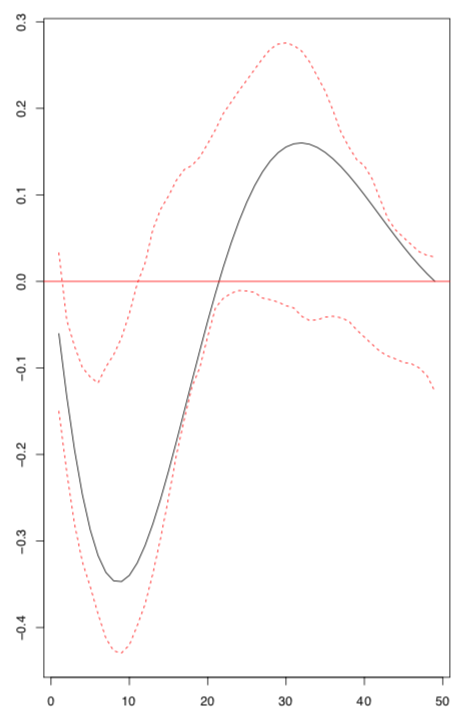
\includegraphics[scale=0.4]{irf_var.png}}
	\caption{}\label{figd47}
%	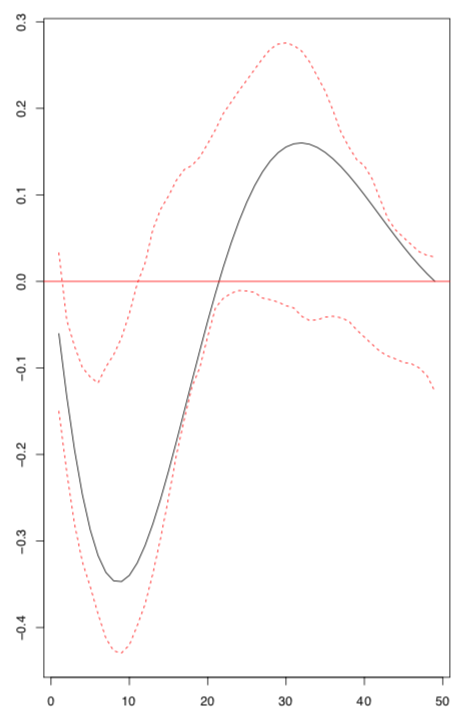
\includegraphics[scale=0.28]{irf_var.pdf}
\end{figure}
%\end{frame}
%---------------------------------------------------------
%---------------------Slide 48--------------------------
%\begin{frame}
%\frametitle{Vector Autoregressive Models}
%\textbf{Ejemplo Modelo VAR - fevd}
\begin{figure}[H]
	\centering
	\textbf{Ejemplo Modelo VAR - fevd}\par\medskip
	\fcolorbox{green}{blue}{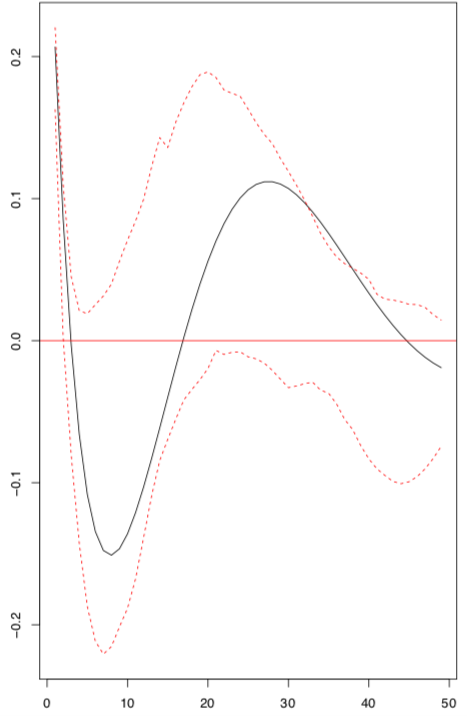
\includegraphics[scale=0.4]{fevd_var.png}}
	\caption{}\label{figd48}
%	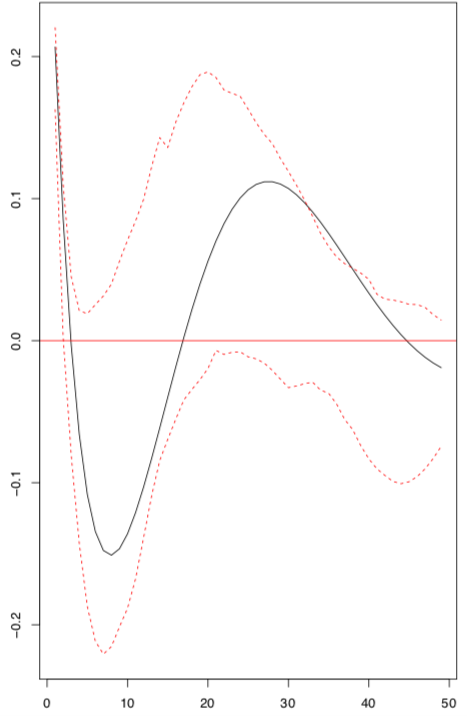
\includegraphics[scale=0.28]{fevd_var.pdf}
\end{figure}
%\end{frame}
%---------------------------------------------------------
%---------------------Slide 49--------------------------
%\begin{section}{Significancia de un Block y Test de Causalidad}
%\begin{frame}
%	\frametitle{Vector Autoregressive Models}
\subsection{Significancia de un Block y Test de Causalidad}
	
%	\textbf{Significancia de un Block y Test de Causalidad}
	
	Es probable que, cuando un modelo VAR incluye muchos rezagos de las variables, sea dif\'{i}cil ver qu\'e conjuntos de variables tienen efectos significativos sobre cada variable dependiente y cu\'ales no. Por ejemplo, considere la siguiente VAR(3) bivariado:
	\scriptsize
	\begin{gather*}
	\begin{pmatrix} y_{1t} \\ y_{2t} \end{pmatrix}
	\begin{pmatrix} \alpha_{10} \\ \alpha_{20} \end{pmatrix}
	+
	\begin{pmatrix} \beta_{11} & \beta_{12} \\ \beta_{21} & \beta{22} \end{pmatrix}
	\begin{pmatrix} y_{1t-1} \\ y_{2t-1} \end{pmatrix}
	+
	\begin{pmatrix} \gamma_{11} & \gamma_{12} \\ \gamma_{21} & \gamma{22} \end{pmatrix}
	\begin{pmatrix} y_{1t-2} \\ y_{2t-2} \end{pmatrix}
	+
	\begin{pmatrix} \delta_{11} & \delta_{12} \\ \delta_{21} & \delta{22} \end{pmatrix}
	\begin{pmatrix} y_{1t-3} \\ y_{2t-3} \end{pmatrix}
	+
	\begin{pmatrix} \mu_{1t} \\ \mu_{2t} \end{pmatrix}
	\end{gather*}
	
	
	Este VAR puede ser escrito para expresar las ecuaciones individuales como:
	\footnotesize
	\begin{equation*}
	y_{1t} = \alpha_{10} + \beta_{11} y_{1t-1} + \beta_{12} y_{2t-1} + \gamma_{11} y_{1t-2} + \gamma_{12} y_{2t-2} + \delta_{11} y_{1t-3} + \delta_{12} y_{2t-3} + \mu_1t
	\end{equation*}
	\begin{equation*}
	y_{2t} = \alpha_{20} + \beta_{21} y_{1t-1} + \beta_{22} y_{2t-1} + \gamma_{21} y_{1t-2} +\gamma_{22} y_{2t-2} + \delta_{21} y_{1t-3} + \delta_{22} y_{2t-3} + \mu_2t
	\end{equation*}
	
%\end{frame}
%---------------------------------------------------------
%---------------------Slide 50--------------------------
%\begin{frame}
%	\frametitle{Vector Autoregressive Models}
%	\textbf{Significancia de un Block y Test de Causalidad}\\
	
	Podr\'{i}amos estar interesados en probar las siguientes hip\'otesis, y sus restricciones impl\'{i}citas en las matrices de par\'ametros:\\
	\begin{figure}[H]
		\fcolorbox{green}{blue}{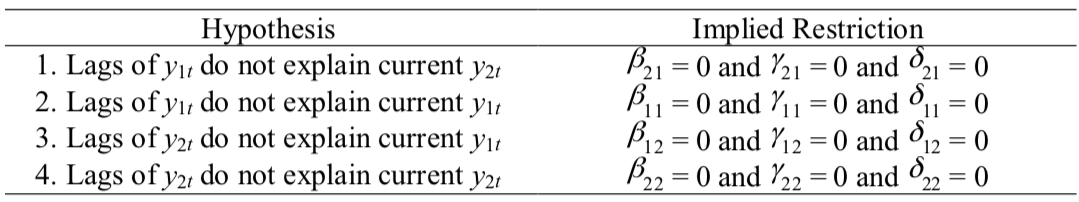
\includegraphics[width=\linewidth]{causality.png}}
	\end{figure}
	
	Cada una de estas cuatro hip\'otesis conjuntas pueden ser probadas usando un test F, ya que cada conjunto de restricciones s\'olo contiene los par\'ametros extra\'{i}dos de una ecuaci\'on.\\
	
	Estas pruebas tambi\'en pueden ser llamadas Pruebas de Causalidad de Granger.\\
	
%\end{frame}
%---------------------------------------------------------
%---------------------Slide 51--------------------------
%\begin{frame}
%	\frametitle{Vector Autoregressive Models}
%	
%	\textbf{Significancia de un Block y Test de Causalidad}\\
	Las \textbf{pruebas de causalidad de Granger} tratan de responder a preguntas como ?`Los cambios en $y_1$ causan cambios en $y_2$?.\\
	\textbf{Si $y_1$ causa $y_2$, rezagos de $y_1$ deber\'{i}an ser significativos en la ecuaci\'on $y_2$. Si este es el caso, se dice que $y_1$ ``Granger-causa" $y_2$. ($y_1$ ``Granger-causes” $y_2$)}\\
	
	\textbf{Si $y_2$ causa $y_1$, retardos de $y_2$ deben ser significativos en la ecuaci\'on de $y_1$.}\\
	
	Si ambos conjuntos de rezagos son importantes, existe una ``relaci\'on de causalidad bidireccional".\\
	
%\end{frame}
%\end{section}
%---------------------------------------------------------
%---------------------Slide 52--------------------------
%\begin{frame}
%\frametitle{Vector Autoregressive Models}
%\textbf{Ejemplo Modelo VAR - Test de Causalidad de Granger}

%\only<1|handout:1>{
%	\begin{exampleblock}{C\'odigo en R}
%		
%		var.cg $<-$ VAR(Canada, p = 2, type = ``const") \\
%		causality(var.cg, cause = ``e")\\
%		grangertest(prod $\string ~$ e, order=4)\\
%		\vspace{3mm}	
%		for (i in 1:4)\\
%		\{\\
%		cat("LAG =", i)\\
%		print(causality(VAR(mydata, p = i, type = ``const"), cause = ``e")$Granger)\\
%		\}\\
%		
%	\end{exampleblock}
%}
\lstset{caption=framexleftmargin=5mm, frame=shadowbox, rulesepcolor=\color{green}}
\begin{lstlisting}[title={‘Código R: Ejemplo Modelo VAR - Test de Causalidad de Granger},basicstyle=\ttfamily]{}
var.cg <-VAR(Canada, p = 2, type = "const")
causality(var.cg, cause = "e")
grangertest(prod~e,order=4,data=Canada)
for (i in 1:4){
cat("LAG =", i)
print(causality(VAR(Canada, p = i, type = "const"), cause ="e")$Granger)
}
\end{lstlisting}
%\end{frame}

%---------------------------------------------------------
%---------------------Slide 53-------------------------
%\begin{frame}
%\frametitle{Vector Autoregressive Models}
%\textbf{Ejemplo Modelo VAR - Test de Causalidad de Granger}

\begin{figure}[H]
		\centering
		\textbf{Test de granger sobre la variable \textquotedblleft prod \textquotedblright}\par\medskip
		\fcolorbox{green}{blue}{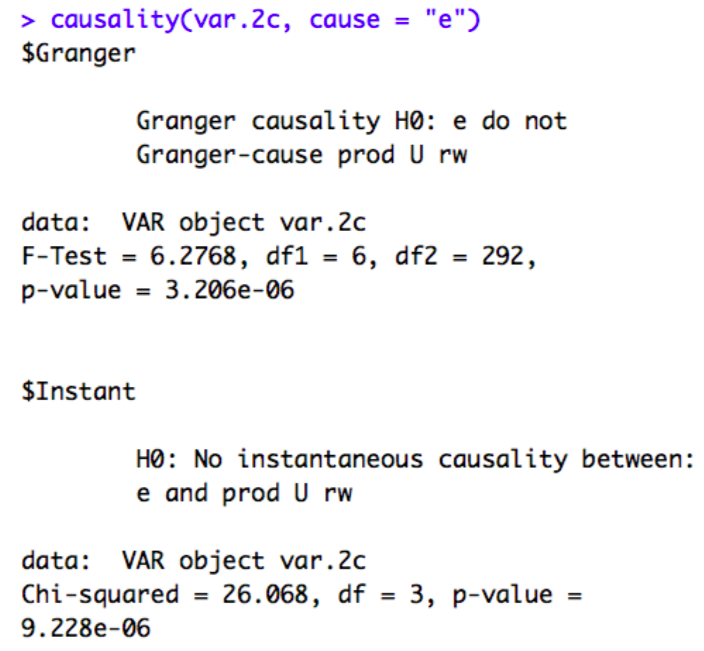
\includegraphics[scale=0.5]{granger.png}}
		\caption{Resultados de test de causalidad de Granger: Ho: \textquotedblleft e\textquotedblright no es Granger-Causa de \textquotedblleft prod\textquotedblright, es decir los rezagos de \textquotedblleft e\textquotedblright no son significativos en la ecuación de \textquotedblleft prod\textquotedblright}\label{figd53}
%	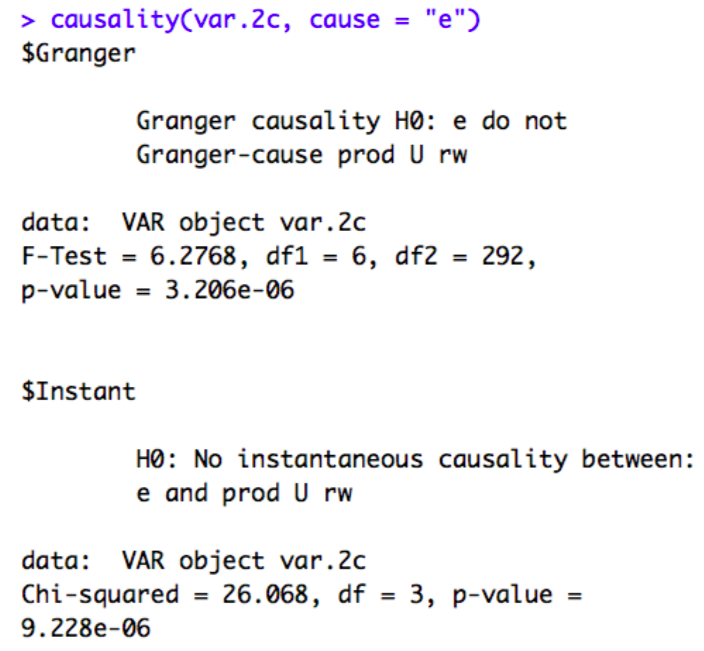
\includegraphics[scale=0.4]{granger.png}
\end{figure}

%\end{frame}

%---------------------------------------------------------
%---------------------Slide 54--------------------------
%\begin{frame}
%\frametitle{Vector Autoregressive Models}
%
%\textbf{Resumen}
\subsection{Resumen}

%\only<1->{
	\begin{itemize}
		\item Hasta ahora hab\'{i}amos estudiado modelos univariados.
		\item Ventajas del modelo VAR: a) es relativamente f\'acil de especificar y de estimar, b) las variables pueden ser no-estacionarias, c) los errores pueden estar correlacionados contempor\'aneamente.
		\item Desventajas del modelo VAR: muchos p\'arametros.
		\item Así, en este t\'opico ampliamos nuestro entendimiento de la relaci\'on entre series de tiempo, permitiendo la posibilidad que exista retroalimentación a partir de shocks idiosincr\'aticos. 
		\item Esta din\'amica puede ser capturada por medio de un modelo de vector autorregresivo (VAR), que es fundamentalmente una generalizaci\'on del an\'alisis de procesos autorregresivos, en el cual, en lugar de considerar una sola variable, se considera un vector de variables.
	\end{itemize}
%}

%\end{frame}
%---------------------------------------------------------
%---------------------Slide 55--------------------------

%\begin{section}{Tarea 3}
%\begin{frame}
%	\frametitle{Tarea 3}

%	Calibrar un modelo del tipo VAR, y desarrollar las siguientes actividades:
%	
%	i) Encontrar la ra\'{i}z unitaria de cada variable.
%	ii) Seleccionar los lags \'optimos del modelo.
%	iii) Calibrar el modelo e interpretar sus resutados.
%	iv) Analizar los residuos y la estabilidad de su modelo.
%	v) Realizar un análisis de impulso y descomposici\'{i}n de varianza.
%	vi) Realizar pron\'ostico extra-muestral usando ventanas m\'oviles.
%	vii) Comparar los errores de su modelo, con el mejor modelo univariado que pueda desarrollar (recuerde tarea 2).
%	
%	\vspace{4mm}	
%	Basarse en paper anexo.
	
\pagebreak
\section{Tarea 3}

\begin{mdframed}[style=MyFrame]
	Calibrar un modelo del tipo VAR, y desarrollar las siguientes actividades:\\
		\textbf{1.} Encontrar la ra\'{i}z unitaria de cada variable.\\
		\textbf{2.} Seleccionar los lags \'optimos del modelo.\\
		\textbf{3.} Calibrar el modelo e interpretar sus resutados.\\
		\textbf{4.} Analizar los residuos y la estabilidad de su modelo.\\
		\textbf{5.} Realizar un análisis de impulso y descomposici\'{i}n de varianza.\\
		\textbf{6.} Realizar pron\'ostico extra-muestral usando ventanas m\'oviles.\\
		\textbf{7.} Comparar los errores de su modelo, con el mejor modelo univariado que pueda desarrollar (recuerde tarea 2).\\
	\vspace{4mm}	
	Basarse en paper anexo.
\end{mdframed}
%\end{frame}
%\end{section}
%---------------------------------------------------------

\curinstructor{Marcelo Villena Chamorro PhD.}